\باب{امالی مشین}
\اصطلاح{قوی برقیات}\فرہنگ{برقیات!قوی}\حاشیہب{power electronics}\فرہنگ{electronics!power} کی میدان میں ترقی کی بنا امالی موٹروں کی رفتار پر قابو رکھنا ممکن ہوا اور یوں ان موٹروں نے کارخانوں میں یک سمت  رو موٹروں کی جگہ لینا شروع کیا۔اس سے پہلے جہاں بھی موٹر کی رفتار اہم  ہوتی وہاں یک سمت  رو موٹر  استعمال ہوتی جن کی رفتار پر قابو رکھنا نہایت آسان ہوتا ہے۔پچاس سال قبل ترقی یافتہ ممالک میں یک سمت موٹر  کی جگہ  امالی موٹر کا استعمال شروع ہوا۔ آج میں یہی تبدیلی پاکستان میں دیکھ رہا ہوں۔ امالی موٹروں کی مضبوطی اور دیرپا کام کرنے کی صلاحیت مثالی ہے۔ قوی الیکٹرانکس نے ان کی رفتار کو قابو کر کے  بلا مقابلہ بنا دیا۔

امالی موٹر درحقیقت  ٹرانسفارمر کی دوسری صورت ہے یا یوں کہنا بہتر ہو گا کہ یہ ایک ایسا ٹرانسفارمر ہے جس کا ثانوی لچھا حرکت بھی کرتا ہے۔یوں امالی موٹر کے ساکن لچھے ٹرانسفارمر کے ابتدائی لچھے اور موٹر کے گھومتے لچھے ٹرانسفارمر کے ثانوی لچھے تصور کیے جا سکتے ہیں۔موٹر کے ساکن لچھوں کو بیرونی برقی طاقت فراہم کی جاتی ہے جبکہ  خلاء میں گھومتے مقناطیسی موج سے پیدا گھومتے لچھوں میں امالی برقی دباو  ان لچھوں کو طاقت فراہم کرتا ہے۔اسی کی بنا ان کو \اصطلاح{امالی موٹر}\فرہنگ{موٹر!امالی}\حاشیہب{induction motor}\فرہنگ{induction!motor} کہتے ہیں

 اس باب کا مقصد امالی موٹر کے مساوی دور  (\اصطلاح{ریاضی نمونہ})\فرہنگ{ریاضی نمونہ}\حاشیہب{mathematical model}\فرہنگ{model} کا حصول اور موٹر کی خواص پر غور کرنا ہے۔ہم دیکھیں گے کہ ان کا مساوی دور ٹرانسفارمر کے مساوی دور کی طرح  ہو گا۔

ہم فرض کریں گے کہ موٹر دو قطبی، تین دوری،  ستارہ  جڑی ہے۔اس طرح یک دوری لچھوں کا برقی رو، تار برقی رو ہو گا اور  یک دوری برقی دباو
 \عددی{\tfrac{\hat{V}_{\text{تار}}}{\sqrt{3}}} ہو گا۔ایسا کرنے سے مسئلے پر غور کرنا آسان ہو گا جبکہ نتیجہ کسی بھی موٹر کے لئے کارآمد ہو گا۔

\حصہ{ساکن لچھوں کی گھومتی مقناطیسی موج}
امالی مشین کے ساکن لچھے بالکل معاصر مشین کے ساکن لچھوں کی طرح ہوتے ہیں۔مزید  گھومتے حصہ اور ساکن لچھوں کے قطبین کی تعداد ایک جیسی ہو گی ۔ساکن لچھوں کو متوازن تین دوری برقی رو سے ہیجان  کرنے سے گھومتے مقناطیسی دباو کی ایک  موج پیدا ہو گی۔ مساوات  \حوالہ{مساوات_تبادلہ_گھومتا_موج} اس موج کو ظاہر کرتی ہے جبکہ مساوات \حوالہ{مساوات_گھومتے_مشین_برقی_میکانی_رفتار_تعلق}  اس کی معاصر رفتار  دیتی ہے جس کو یہاں \عددی{f_s} لکھا گیا ہے۔یہ دونوں مساوات یہاں یاد دھیانی کے لئے دوبارہ پیش کرتے  ہیں۔یہاں ساکن لچھوں میں برقی رو کا تعدد \عددیء{\omega_e} لکھا گیا ہے اور \عددیء{\alpha}  صفر لیا گیا ہے۔
\begin{gather}
\begin{aligned}\label{مساوات_امالی_گھومتا_مقناطیسی_دباو_الف}
\tau_s^+ (\theta,t)&=\frac{3 \tau_0}{2} \cos (\theta-\omega_ e t)\\
f_s&=\frac{2}{P} f_e
\end{aligned}
\end{gather}

\حصہ{مشین کا سرکاو اور گھومتی امواج پر تبصرہ}
ہم دو قطب کی مشین پر غور کر رہے ہیں جو \عددیء{P} قطبی مشین کے لئے بھی درست ہے۔ساکن لچھوں میں تین دوری برقی رو کا تعدد \عددیء{f_e} ہے۔مساوات \حوالہ{مساوات_گھومتے_مشین_برقی_میکانی_رفتار_تعلق}  کہتی ہے کہ دو قطبی مشین میں موج کی معاصر رفتار بھی \عددیء{f_e} چکر فی سیکنڈ ہو گی۔ اب تصور کریں مشین کا گھومتا حصہ، \عددیء{f} میکانی چکر فی سیکنڈ کی رفتار سے موج کے رخ گھوم رہا ہے جہاں \عددیء{f<f_s} ہے۔ یوں ہر سیکنڈ گھومتا حصہ مقناطیسی بہاو کی موج سے \عددی{f_s-f} پیچھے سرک جائے گا۔اس سرکنے کو موج کی معاصر رفتار کی نسبت سے درج ذیل لکھا جاتا ہے۔
\begin{align}
s&=\frac{f_s-f}{f_s}=\frac{f_e-f}{f_e}
\end{align}
یہاں \عددیء{s} مشین کے سرکاو\فرہنگ{سرکاو}\حاشیہب{slip}\فرہنگ{slip} کی ناپ ہے۔اس مساوات سے درج ذیل حاصل ہو گا۔
\begin{gather}
\begin{aligned}\label{مساوات_امالی_سرک_اور_تعدد}
f&=f_s (1-s)=f_e(1-s)\\
\omega&=\omega_s(1-s)=\omega_e(1-s)&&\text{\RL{\small{(\عددی{2\pi} سے ضرب دیا گیا ہے)}}}
\end{aligned}
\end{gather}
یہاں غور کیجیے گا۔ مقناطیسی بہاو کی موج \عددیء{f_e} تعدد سے گھوم رہی ہے جبکہ  گھومتا لچھا \عددیء{f} تعدد سے گھوم رہا ہے۔گھومتے لچھا کے حوالہ سے مقناطیسی بہاو کی موج \عددیء{(f_e-f)} رفتار سے گھوم رہی ہے، یعنی،  گھومتے لچھے کو ساکن تصور کرنے سے  گھومتے مقناطیسی بہاو کی موج \عددیء{(f_e-f)} اضافی رفتار سے گھومتی نظر آئے گی۔یوں گھومتے لچھا میں امالی برقی دباو کا تعدد بھی \عددیء{(f_e-f)} ہو گا۔مساوات \حوالہ{مساوات_امالی_سرک_اور_تعدد}  کی مدد سے اس امالی برقی دباو کا (اضافی) تعدد \عددیء{f_z}  درج ذیل  لکھا جا سکتا ہے۔
\begin{align}\label{مساوات_امالی-سرک_تعلق_ب}
f_z=f_e-f=f_e-f_e(1-s)=s f_e
\end{align}
مشین بطور امالی موٹر استعمال کرنے کے لئے  گھومتے لچھے کسر دور کیے جائیں گے۔ان کسر دور  لچھوں میں برقی رو کا تعدد \عددیء{s f_e} اور رو کی قیمت لچھوں میں پیدا امالی برقی دباو اور لچھوں کی رکاوٹ پر منحصر ہو گی۔ لچھوں کی رکاوٹ برقی رو کے تعدد پر منحصر ہو گی۔

ساکن موٹر جب چالو کی جائے تو اس کا سرکاو \عددیء{s}   اکائی (\عددی{s=1}) ہو گا لہٰذا  گھومتے لچھوں میں برقی رو کا تعدد \عددیء{f_e} ہو گا۔ گھومتے لچھوں میں \عددیء{f_e}  تعدد کا برقی رو ایک گھومتی مقناطیسی دباو کی موج پیدا کرے گا جو معاصر رفتار سے گھومے گی۔یہ بالکل اسی طرح ہے جیسا ساکن لچھوں میں برقی رو سے گھومتے مقناطیسی دباو کی موج وجود میں آتی ہے۔یوں موٹر چالو کرنے کے  لمحہ پر ساکن اور گھومتے لچھوں کے  مقناطیسی دباو کی امواج ایک جیسی رفتار سے گھومتی ہیں۔مقناطیسی دباو کی یہ امواج  دو گھومتے مقناطیسوں کی طرح  کوشش کرتی ہیں کہ ان کے بیچ زاویہ صفر ہو۔یوں موٹر \اصطلاح{قوت مروڑ}\فرہنگ{قوت مروڑ}\حاشیہب{torque}\فرہنگ{torque} پیدا کرتی  ہے جسے  مساوات \حوالہ{مساوات_گھومتے_مشین_مروڑ_بذریعہ_کوتوانائی_الف} میں پیش کیا گیا ہے۔اگر موٹر کے دھرے پر لدے بوجھ کو مشین کی پیدا کردہ قوت مروڑ گھما سکے تو مشین گھومے گی۔اس کی رفتار تیز ہو کر ایک برقرار حد تک پہنچ جائے گی۔ امالی موٹر کی رفتار کبھی بھی معاصر رفتار تک نہیں پہنچ سکتی چونکہ اس رفتار پر اس کے گھومتے لچھوں کی نسبت سے ساکن لچھوں کی گھومتی مقناطیسی دباو کی موج ساکن ہو گی اور گھومتے لچھوں میں کوئی امالی برقی دباو پیدا نہیں ہو گا۔

جب موٹر چل پڑتی ہے تو اس کے گھومتے لچھوں کے برقی رو کا تعدد \عددیء{s f_e} ہو گا۔ان برقی رو سے پیدا مقناطیسی دباو کی موج گھومتے لچھے کے حوالہ سے \عددیء{s f_e} رفتار سے گھومے گی۔اب گھومتا لچھا از خود  رفتار \عددیء{f}  سے گھوم رہا ہو گا لہٰذا یہ موج درحقیقت خلاء میں \عددیء{(f+s f_e)} رفتار سے گھومے گی۔مساوات \حوالہ{مساوات_امالی-سرک_تعلق_ب}  سے درج ذیل لکھا جا سکتا ہے جو ایک اہم نتیجہ ہے۔
\begin{align}
f+s f_e=f +f_e-f=f_e
\end{align} 
 یہ مساوات کہتی ہے کہ موٹر جس رفتار سے بھی گھوم رہی ہو، گھومتے لچھوں سے پیدا مقناطیسی دباو کی موج ساکن لچھوں سے پیدا مقناطیسی دباو کی موج کی رفتار سے ہی گھومے گی۔
%
\ابتدا{مثال}
ایک چار قطب، ستارہ، \عددیء{50} ہرٹز، \عددیء{415} وولٹ  پر چلنے والی امالی موٹر \عددیء{15} کلو واٹ کی (پوری) بناوٹی بوجھ پر پانچ فی صد سرکاو پر چلتی ہے۔
\begin{itemize}
\item
اس موٹر کی معاصر رفتار کتنی گی؟
\item
پورے بوجھ پر اس کی رفتار کتنی ہو گی؟
\item
پورے بوجھ پر گھومتے لچھے میں برقی تعدد کتنا ہو گا؟
\item
پورے بوجھ سے لدے موٹر کی دھرے پر قوت مروڑ کتنی ہو گی؟
\end{itemize}

حل:
\begin{itemize}
\item
مساوات \حوالہ{مساوات_امالی_گھومتا_مقناطیسی_دباو_الف}  کی مدد سے معاصر رفتار \عددیء{f_m=\tfrac{2}{4}\times 50=25} چکر فی سیکنڈ یا \عددیء{25 \times 60=1500} چکر فی منٹ ہو گی۔
\item
پورے بوجھ سے لدی موٹر پانچ فی صد سرکاو پر چلتی ہے لہٰذا اس کی رفتار معاصر رفتار سے  کم ہو گی۔موٹر کی رفتار مساوات \حوالہ{مساوات_امالی_سرک_اور_تعدد}   کی مدد سے \عددیء{f=25 (1-0.05)=23.75} چکر فی سیکنڈ یا \عددیء{1425} چکر فی منٹ حاصل ہوتی ہے۔
\item
گھومتے لچھے کا برقی تعدد  \عددیء{f_r=0.05 \times 50=2.5} ہرٹز ہو گا۔
\item
اس کے دھرے پر قوت مروڑ \عددیء{T_m=\tfrac{p}{\omega_m}=\tfrac{15000}{2 \times \pi \times 23.75}=\SI{100.5}{\newton \meter}} ہو گی۔
\end{itemize}
\انتہا{مثال}
%
\حصہ{ساکن لچھوں میں امالی برقی دباو}
مساوات \حوالہ{مساوات_امالی_گھومتا_مقناطیسی_دباو_الف}  کا پہلا جزو ساکن لچھوں کی پیدا کردہ مقناطیسی دباو کی موج  کو ظاہر کرتا ہے۔یہ مقناطیسی دباو مشین کی خلائی درز میں مقناطیسی شدت \عددیء{H^+(\theta)} پیدا کرے گی جس سے درز میں  کثافت مقناطیس بہاو \عددیء{B^+(\theta)} پیدا ہو گا۔ خلائی درز کی رداسی رخ  لمبائی \عددیء{l_g} لیتے ہوئے درج ذیل ہو گا
\begin{gather}
\begin{aligned}\label{مساوات_امالی-سرک_تعلق_پ}
B^+(\theta)=\mu_0 H^+(\theta)&=\mu_0 \frac{\tau^+(\theta)}{l_g}\\
&=\frac{3 \mu_0 \tau_0}{2 l_g} \cos (\theta-\omega_e t)\\
&=B_0 \cos (\theta-\omega_e t)
\end{aligned}
\end{gather}
جو بالکل مساوات \حوالہ{مساوات_گھومتے_مشین_کثافت_بالمقابل_میکانی_زاویہ}  کی طرح ہے۔درج بالا میں \عددی{B_0=\tfrac{3\mu_0\tau_0}{2l_g}} لیا گیا ہے۔ یوں مساوات \حوالہ{مساوات_گھومتے_مشین_تین_دور_سائن_نما_برقی_دباو}   مقناطیسی موج \عددیء{B^+(\theta)} کی ساکن لچھوں میں پیدا کردہ امالی برقی دباو کو ظاہر کرے گی ۔اس مساوات کو یہاں دوبارہ پیش کیا جاتا ہے
\begin{gather}
\begin{aligned}\label{مساوات_امالی_تین_دور_سائن_نما_برقی_دباو}
e_{as}(t)&=\omega_e N_s \phi_0 \cos (\omega_t +90\degree)=E_s \cos (\omega_t +90\degree)\\
e_{bs}(t)&=\omega_e N_s \phi_0 \cos (\omega_t -30\degree)=E_s \cos (\omega_t -30\degree)\\
e_{cs}(t)&=\omega_e N_s \phi_0 \cos (\omega_t +210\degree)=E_s \cos (\omega_t +210\degree)
\end{aligned}
\end{gather}
جہاں \عددیء{N_s} ساکن لچھے کے چکر  اور \عددی{E_s} درج ذیل ہے۔
\begin{align}
E_s=\omega_e N_s \phi_0
\end{align}
یہاں \عددیء{e_{as}(t)}  لکھتے ہوئے  زیر نوشت  میں \عددیء{a} ،  دور \عددیء{a} کو ظاہر کرتا ہے اور \عددیء{s}، ساکن\حاشیہد{لفظ ساکن میں حرف س کے آواز کو \عددیء{s} سے ظاہر کیا گیا ہے۔} کو ظاہر کرتا ہے یعنی یہ ساکن \عددیء{a}  لچھے کا امالی برقی دباو ہے۔امالی موٹر کے  دور \عددیء{a}  کی بات آگے بڑھاتے ہیں۔گھومتی مقناطیسی دباو کی موج اس  لچھے میں امالی برقی دباو \عددیء{e_{as}(t)} پیدا کرتی ہے۔

\حصہ{ساکن لچھوں کی  موج کا گھومتے لچھوں کے ساتھ اضافی رفتار اور ان میں پیدا امالی برقی دباو}
ساکن لچھوں کی پیدا کردہ، گھومتے مقناطیسی دباو کی موج (مساوات \حوالہ{مساوات_امالی_گھومتا_مقناطیسی_دباو_الف})  کی چوٹی\فرہنگ{چوٹی}\حاشیہب{peak} اس مقام پر ہو گی جہاں \عددیء{(\theta-\omega_e t)} صفر کے برابر ہو۔ یوں لمحہ صفر پر اس کی چوٹی صفر زاویہ
 \عددی{(\theta=0)} پر ہو گی اور لمحہ \عددیء{t} پر اس موج کی چوٹی زاویہ \عددیء{\omega_e t} پر ہو گی۔ ساکن لچھوں کی مقناطیسی دباو کی موج کا زاویہ کسی بھی نقطہ کے حوالے سے ناپا  جا سکتا ہے۔ اس کتاب میں ساکن لچھا \عددیء{a}  کو صفر زاویہ تصور کیا گیا ہے۔یوں شکل \حوالہ{شکل_امالی_گھومتی_موجیں}  میں  نقطہ دار افقی لکیر سے  زاویہ   ناپا جائے گا۔اس شکل میں ایک امالی موٹر دکھائی گئی ہے جس کے  ساکن لچھے تین دوری ہیں۔
\begin{figure}
\centering
%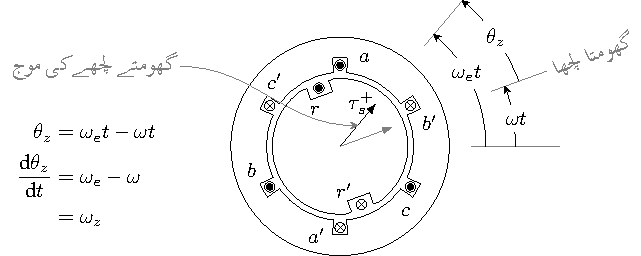
\includegraphics{figInductionStatorAndRotorWaves}
\begin{tikzpicture}
%grid
%\draw[gray] (-\sRo,-\sRo) grid (\sRo,\sRo);
\pgfmathsetmacro{\shiftX}{5cm}
\stator{6}{30}
\slotDot{90,-30,210}
\slotCross{-90,30,150}
\pgfmathsetmacro{\pTheta}{50}
\pgfmathsetmacro{\pY}{0.2}
\pgfmathsetmacro{\rTilt}{20}
\rotor{6}{\rTilt}
\draw node at (\rTilt+90+20:\rR-0.4){$a_r$};
\draw node at (\rTilt+90+180+22:\rR-0.4){$a_r'$};
%dot on rotot
\draw (90+\rTilt:\rR-3*\pX) circle (2.5pt);
\draw[fill] (90+\rTilt:\rR-3*\pX) circle (1.5pt);
\draw (90+120+\rTilt:\rR-3*\pX) circle (2.5pt);
\draw[fill] (90+120+\rTilt:\rR-3*\pX) circle (1.5pt);
\draw (90+240+\rTilt:\rR-3*\pX) circle (2.5pt);
\draw[fill] (90+240+\rTilt:\rR-3*\pX) circle (1.5pt);
%CROSS on rotor
\draw (\rTilt-90:\rR-3*\pX) circle (2.5pt);
\draw (\rTilt-90:\rR-3*\pX)++(45:2.2pt)--++(-135:4.4pt);
\draw (\rTilt-90:\rR-3*\pX)++(-45:2.2pt)--++(135:4.4pt);
\draw (\rTilt-90+120:\rR-3*\pX) circle (2.5pt);
\draw (\rTilt-90+120:\rR-3*\pX)++(45:2.2pt)--++(-135:4.4pt);
\draw (\rTilt-90+120:\rR-3*\pX)++(-45:2.2pt)--++(135:4.4pt);
\draw (\rTilt-90+240:\rR-3*\pX) circle (2.5pt);
\draw (\rTilt-90+240:\rR-3*\pX)++(45:2.2pt)--++(-135:4.4pt);
\draw (\rTilt-90+240:\rR-3*\pX)++(-45:2.2pt)--++(135:4.4pt);
%mmf vector and angles
\draw[-latex,gray] (0,0)--(\rTilt:0.8*\rR);
\draw[-latex](0,0)-- (\rTilt+40:0.45*\rR)coordinate[pos=0.5](statorMMF)node[above,pos=0.8,font=\small]{$\tau_s^+$};
\draw[gray](0:1.2*\sRo)--++(0:1.5cm);
\draw[](\rTilt:1.2*\sRo cm +0.5cm)--++(\rTilt:1cm)node [right,rotate=\rTilt]{\RL{گھومتا \عددی{r_a} لچھا}};
\draw[gray] (\rTilt+40:1.2*\sRo) --++(\rTilt+40:1cm) ;
%\draw[](statorMMF)++(-0.05,0) to [out=180,in=0] ++(-3,1)node[left]{\RL{گھومتے لچھوں کی موج}};
\draw node[left] at (-3,-0.5){$
\begin{aligned}
\theta_z&=\omega_e t - \omega t\\
\frac{\textup{d} \theta_z}{\textup{d} t}&=\omega_e-\omega\\
&=\omega_z
\end{aligned}
$};
%
\draw[-stealth] (0:1.2*\sRo cm +0.75 cm)  arc (0:\rTilt:1.2*\sRo cm +0.75 cm);
\draw node[right,fill=white] at (\rTilt/2:1.2*\sRo cm+0.5 cm){$\omega t$}; 
%
\draw[-stealth] (\rTilt:1.2*\sRo cm +0.9 cm)  arc (\rTilt:\rTilt+40:1.2*\sRo cm +0.9 cm);
\draw node[fill=white] at (\rTilt+20:1.2*\sRo+0.9){$\theta_z$};
%
\draw[-stealth] (0:1.2*\sRo cm +0.25 cm)  arc (0:\rTilt+40:1.2*\sRo cm +0.25 cm);
\draw node[fill=white] at (\rTilt/2+20:1.2*\sRo cm+0.25 cm){$\omega_e t$};
%\slotName{45/a_1/,-45/a_1'/below,135/a_2'/,-135/a_2/below}
\draw (90-15:\sRi+1.25*\delR)node[]{$a$};
\draw (270-15:\sRi+1.25*\delR)node[]{$a'$};
\draw (210-15:\sRi+1.25*\delR)node[]{$b$};
\draw (30-15:\sRi+1.25*\delR)node[]{$b'$};
\draw (-30-15:\sRi+1.25*\delR)node[]{$c$};
\draw (150-15:\sRi+1.25*\delR)node[]{$c'$};
\end{tikzpicture}
\caption{امالی موٹر اور اس کے گھومتے مقناطیسی دباو کی موجیں۔}
\label{شکل_امالی_گھومتی_موجیں}
\end{figure}

مشین \عددیء{f} زاویائی رفتار سے گھوم رہی ہے۔ تصور کریں کہ لمحہ صفر یعنی \عددیء{t=0} پر گھومتے حصہ کا  \عددیء{a_r} لچھا صفر زاویہ پر ہے، یعنی یہ نقطہ دار افقی لکیر پر ہے۔ مزید تصور کریں کہ اس لمحہ ساکن لچھوں کی گھومتی مقناطیسی دباو کی موج بھی اسی افقی لکیر پر ہے۔ اب کچھ دیر بعد لمحہ \عددیء{t} پر یہ موج زاویہ  \عددیء{\omega_e t} پر ہو گی۔ اتنی دیر میں گھومتا حصہ گھوم کر زاویہ  \عددیء{\omega t} تک پہنچے گا جہاں \عددیء{\omega=2 \pi f}  مشین کی زاویائی میکانی رفتار ہے۔یہ سب شکل \حوالہ{شکل_امالی_گھومتی_موجیں} میں دکھایا گیا ہے۔لہٰذا لمحہ \عددیء{t} پر موج اور گھومتے لچھے کے بیچ زاویہ \عددیء{\theta_z} درج ذیل ہو گا۔
\begin{align}
\theta_z=\omega_e t -\omega t
\end{align}
اگرچہ مقناطیسی موج نے \عددیء{\omega_e t} زاویہ طے کیا لیکن گھومتے لچھے کے حوالے سے اس نے صرف  زاویہ \عددیء{(\omega_e t -\omega t)} طے کیا۔گھومتے لچھے کے حوالے سے  موج کی  اضافی\حاشیہد{\عددیء{\omega_z} لکھتے ہوئے زیر نوشت میں \عددیء{z}،  لفظ اضافی کے حرف ض کی آواز کو ظاہر کرتا ہے۔} زاویائی رفتار\فرہنگ{اضافی!زاویائی رفتار}\فرہنگ{رفتار!اضافی زاویائی}\حاشیہب{relative angular speed} \عددیء{\omega_z} درج ذیل ہو گی
\begin{align}
\omega_z=\frac{\dif \theta_z}{\dif t}=\omega_e -\omega
\end{align}
جس کو مساوات \حوالہ{مساوات_امالی-سرک_تعلق_ب} کی مدد سے درج ذیل لکھا جا سکتا ہے۔
\begin{align}
\omega_z=2 \pi (f_e-f)=2 \pi s f_e = s \omega_e
\end{align}
یہ مساوات کہتی ہے کہ گھومتے لچھوں کے حوالے سے مقناطیسی موج کی رفتار سرکاو \عددیء{s} پر منحصر ہو گی۔البتہ اس موج کا حیطہ  تبدیل نہیں ہوا۔ یوں گھومتے لچھوں کے حوالہ سے مساوات \حوالہ{مساوات_امالی-سرک_تعلق_پ} درج ذیل صورت اختیار کرتی ہے۔
\begin{align}
B_{s,rz}^+(\theta,t)&=B_0 \cos (\theta-\omega_z t)=B_0 \cos (\theta -s \omega_e t)
\end{align}
\عددیء{B_{s,rz}^+} میں \عددیء{+} کا نشان  خلاف گھڑی موج کو ظاہر کرتا ہے جبکہ  زیر نوشت میں \عددیء{s,rz}  \حاشیہد{\عددیء{s} لفظ ساکن کے س کو ظاہر کرتا ہے ، \عددیء{r} لفظ رواں کے ر کو ظاہر کرتا ہے اور \عددیء{z}  لفظ اضافی کے ض کو ظاہر کرتا ہے۔} اس بات کی یاد دھیانی کرتا ہے کہ یہ موج ساکن لچھوں کی وجہ سے وجود میں آئی  اور اسے گھومتے یعنی رواں لچھوں کے حوالے سے دیکھا جا رہا ہے۔مزید، اس مساوات کا تعدد اضافی تعدد \عددیء{\s \omega_e} کے برابر ہے۔

یوں گھومتے لچھوں میں امالی برقی دباو مساوات \حوالہ{مساوات_امالی_تین_دور_سائن_نما_برقی_دباو}  کی طرح  ہوں گے لیکن  ان میں تعدد \عددیء{\omega_z=s \omega_e t} ہو گا:\حاشیہد{\عددیء{e_{arz}} میں   دور \عددیء{a} ہے۔گھومتے لچھے کو \عددیء{r}  اور اضافی کو \عددیء{z} ظاہر کرتا ہے۔}
\begin{gather}
\begin{aligned}\label{مساوات_امالی_گھومتا_حصہ_تین_دور_سائن_نما_برقی_دباو}
e_{arz}(t)&=s \omega_e N_r \phi_0 \cos (s \omega_e t +90\degree)=s E_r \cos (s \omega_e t +90\degree)\\
e_{brz}(t)&=s \omega_e N_r \phi_0 \cos (s \omega_e t -30\degree)= s E_r \cos (s \omega_e t -30\degree)\\
e_{crz}(t)&=s \omega_e N_r \phi_0 \cos (s \omega_e t +210\degree)= s E_r \cos (s \omega_e t +210\degree)
\end{aligned}
\end{gather}
ان مساوات میں \عددیء{N_r}  گھومتے لچھے کے چکر ہیں اور \عددی{E_r} درج ذیل ہے۔
\begin{align}
E_r=\omega_e N_r \phi_0
\end{align}

اب تصور کریں گھومتے لچھوں کو کسر دور کر دیا جاتا ہے۔امالی برقی دباو گھومتے لچھوں میں برقی رو \عددیء{i_{arz}}\حاشیہد{یہاں \عددیء{r} گھومتے لچھے کو ظاہر کرتا ہے اور \عددیء{z} اس بات کی یاد دھیانی کرتا ہے کہ اس برقی رو کا تعدد، اضافی تعدد ہے۔}،  وغیرہ،  پیدا کرے گا جس کا تعدد \عددیء{s \omega_e} ہو گا۔ساکن لچھے کی طرح، گھومتے لچھے کی مزاحمت \عددیء{R_r}\حاشیہد{ٹرانسفارمر کی اصطلاح میں ثانوی لچھے  کو زیر نوشت میں \عددیء{2} سے ظاہر کرتے ہیں۔یہاں اسے \عددیء{r} سے ظاہر کیا جاتا ہے۔}  اور  امالہ \عددیء{L_r} یعنی  متعاملیت \عددیء{j s \omega_e L_r} ہو گی:
\begin{align}
j s \omega_e L_r = j s  X_r
\end{align}
یہاں \عددیء{j \omega_e L_r}  کو  \عددیء{j X_r} لکھا گیا ہے جو گھومتے لچھا کو ساکن \عددی{(s=1)} رکھتے ہوئے  گھومتے لچھے  کی متعاملیت ہے۔گھومتے لچھے کا  برقی رو \عددیء{i_{arz}} شکل \حوالہ{شکل_امالی_گھومتی_لچھوں_کا_مساوی_دور}   سے حاصل کیا جا سکتا ہے جہاں گھومتے  لچھے کا امالی برقی دباو \عددیء{e_{arz}(t)} مساوات \حوالہ{مساوات_امالی_گھومتا_حصہ_تین_دور_سائن_نما_برقی_دباو}   میں پیش کیا گیا ہے۔
\begin{figure}
\centering
%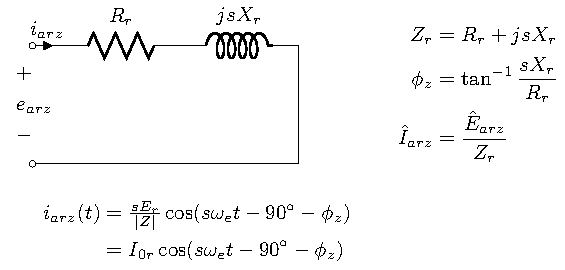
\includegraphics{figInductionRotorEquivalentCircuit}
\begin{tikzpicture}
%grid
%\draw[gray] (-\sRo,-\sRo) grid (\sRo,\sRo);
\pgfmathsetmacro{\shiftX}{5cm}
\draw (0,0) to [short,o-,i={$i_{arz}$}] ++(0.5,0) to [resistor,l={$R_r$}]++(2,0) to [inductor,l={$j s X_{r}$}] ++(2,0) to ++(0,-2) to [short,-o] (0,-2);
\draw node at (0,-1){$\begin{aligned} &+\\ & e_{arz}\\ &- \end{aligned}$};
\draw node[below right] at (6,0.5){$
\begin{aligned}
Z_r&=R_r+j s X_r\\
\phi_z&=\tan^{-1} \frac{s X_r}{R_r}\\
\hat{I}_{arz}&=\frac{\hat{E}_{arz}}{Z_r}
\end{aligned}$};
%
\draw node[below right] at (0,-2.5){$
\begin{aligned}
i_{arz}(t)&=\tfrac{s E_r}{|Z|} \cos (s \omega_e t +90^\circ-\phi_z) \\ 
& =I_{0r} \cos (s \omega_e t +90^\circ-\phi_z) 
\end{aligned}$}; 
\end{tikzpicture}%
\caption{گھومتے لچھا کا مساوی دور اور اس میں اضافی تعدد کا رو۔}
\label{شکل_امالی_گھومتی_لچھوں_کا_مساوی_دور}
\end{figure}

شکل \حوالہ{شکل_امالی_گھومتی_لچھوں_کا_مساوی_دور} بالکل شکل \حوالہ{شکل_حقائق_دوری_سمتیہ_سے_دور_حل}  کی طرح ہے لہٰذا مساوات \حوالہ{مساوات_بنیادی_حقائق_دوری_سمتیہ_سے_مزاحمت_امالہ_دور_حل}  سے برقی رو حاصل کیے جا سکتے ہیں:
\begin{gather}
\begin{aligned}
i_{arz}(t)&=\frac{s E_r}{\sqrt{R_r^2+s^2 X_r^2}} \cos \left(s \omega_e t +90\degree-\phi_z \right)=I_{0r} \cos (s \omega_e t +\theta_0)\\
i_{brz}(t)&=\frac{s E_r}{\sqrt{R_r^2+s^2 X_r^2}} \cos \left(s \omega_e t -30\degree-\phi_z \right)=I_{0r} \cos (s \omega_e t -120 \degree+\theta_0)\\
i_{crz}(t)&=\frac{s E_r}{\sqrt{R_r^2+s^2 X_r^2}} \cos \left(s \omega_e t +210\degree-\phi_z \right)=I_{0r} \cos (s \omega_e t+120\degree +\theta_0)
\end{aligned}
\end{gather}
یہ تین دوری برقی رو ہیں جو آپس میں \عددیء{120\degree}  زاویہ رکھتے ہیں۔یہاں \عددیء{\phi_z} رکاوٹ کا زاویہ\حاشیہد{تکنیکی دنیا میں رکاوٹ کے زاویہ کے لئے \عددیء{\phi_z} استعمال ہوتا ہے۔یہاں یہی کیا گیا ہے۔} ہے۔امید کی جاتی ہے کہ اسے آپ مقناطیسی بہاو نہیں سمجھیں گے۔درج بالا مساوات میں درج ذیل ہوں گے۔
\begin{gather}
\begin{aligned}\label{مساوات_امالی_گھومتا_رو}
\theta_0&=90-\phi_z \\
I_{0r}&=\frac{s E_r}{\sqrt{R_r^2+s^2 X_r^2}}
\end{aligned}
\end{gather}
شکل \حوالہ{شکل_امالی_گھومتی_لچھوں_کا_مساوی_دور}  سے واضح ہے کہ ایک گھومتے لچھے کی مزاحمت میں 
\begin{align}\label{مساوات_امالی_طاقت_ضیاع_گھمتا_حصہ}
p_r =I_{or}^2 R_r
\end{align}
برقی طاقت کا ضیاع ہو گا جہاں (مساوات کی سادہ صورت کی خاطر ہم فرض کرتے ہیں کہ)  \عددی{I_{0r}} برقی رو کی موثر قیمت ہے۔یہ طاقت حرارت میں تبدیل ہو کر  لچھے کو گرم کرے گی۔

\حصہ{گھومتے لچھوں کی گھومتے مقناطیسی دباو کی موج}
ہم جانتے ہیں کہ ساکن تین دوری لچھوں میں \عددیء{f_e} تعدد کے برقی رو   گھومتے مقناطیسی دباو کی موج پیدا کرتے ہیں جو ساکن لچھے کے حوالے سے  \عددیء{f_e} معاصر زاویائی رفتار سے گھومتی ہے۔ اسی طرح گھومتے تین دوری لچھوں میں \عددیء{s f_e} تعدد کے برقی رو ایک گھومتے مقناطیسی دباو کی موج \عددیء{\tau_{rz}^+} پیدا کرتے ہیں جو گھومتے لچھے کے حوالے سے \عددیء{s f_e}  زاویائی رفتار سے گھومتی ہے۔
\begin{align}
\tau_{rz}^+(\theta,t)=k_w \frac{4}{\pi} \frac{N_r I_{0r}}{2} \cos \left(\theta-s \omega_e t -\theta_0 \right)
\end{align}
یہاں  \عددیء{I_{0r}} اور \عددیء{\theta_0} مساوات \حوالہ{مساوات_امالی_گھومتا_رو} میں دیے گئے ہیں۔گھومتا لچھا از خود \عددیء{f} زاویائی رفتار سے گھوم رہا ہو گا لہٰذا اس کی پیدا کردہ  موج خلائی درز  میں \عددیء{(f+s f_e)} زاویائی رفتار سے گھومے گی۔ اس رفتار کو مساوات \حوالہ{مساوات_امالی_سرک_اور_تعدد}  کی مدد سے درج ذیل لکھا جا سکتا ہے۔
\begin{align}
f+s f_e= f_e (1-s)+ s f_e=f_e
\end{align}
یوں  گھومتے لچھوں کے مقناطیسی دباو کی موج کو ساکن لچھوں کے حوالے درج ذیل لکھا جا سکتا ہے۔
\begin{align}\label{مساوات_امالی_گھومتے_حصے_کی_موج}
\tau_{r,s}^+(\theta,t)=k_w \frac{4}{\pi} \frac{N_r I_{0r}}{2} \cos \left(\theta-\omega_e t -\theta_0 \right)
\end{align}
\عددیء{\tau_{r,s}^+} میں \عددیء{+} کا نشان گھڑی کے مخالف رخ گھومتی موج کو ظاہر کرتا ہے جبکہ زیر نوشت  میں \عددیء{r,s} اس بات کی وضاحت کرتا ہے کہ یہ موج گھومتے لچھوں کی وجہ سے وجود میں آیا ہے مگر اسے ساکن لچھوں کے حوالے سے دیکھا جا رہا ہے۔

یہاں ذرا رک کر غور کرتے ہیں۔مساوات \حوالہ{مساوات_امالی_گھومتے_حصے_کی_موج}  کے مطابق گھومتا لچھا خود جس  رفتار سے بھی  گھوم رہا ہو، اس کی پیدا کردہ  موج ساکن لچھے کی پیدا کردہ موج کی رفتار سے ہی گھومے گی۔یوں  مشین میں دو امواج ایک ہی معاصر رفتار سے گھوم رہی ہوں گی۔مساوات \حوالہ{مساوات_گھومتے_مشین_مروڑ_کوتوانائی_سے}  کہتی ہے کہ دو مقناطیسی دباو کی موجیں قوت مروڑ  پیدا کرتی ہیں جو امواج کی چوٹیوں اور ان کے بیچ  زاویہ پر منحصر ہو گی۔امالی مشین میں موجود دو مقناطیسی امواج قوت مروڑ  پیدا کرتی ہیں جس کی قیمت ان  امواج کی چوٹیوں اور ان  کے بیچ زاویہ پر منحصر ہو گی۔امالی موٹر،  لدے بوجھ کے مطابق امواج کے بیچ زاویہ رکھ کر درکار  قوت مروڑ پیدا کرتی ہے۔

\حصہ{گھومتے لچھوں کے مساوی فرضی ساکن لچھے}
اب دوبارہ اصل موضوع پر آتے ہیں۔اگر گھومتے لچھوں کی جگہ \عددیء{N_r} چکر کے تین دوری فرضی ساکن لچھے ہوں تب مساوات \حوالہ{مساوات_امالی_تین_دور_سائن_نما_برقی_دباو}   کی طرح ان میں امالی برقی دباو پیدا ہوں گے:\حاشیہد{ان مساوات میں زیر نوشت میں \عددیء{f} لفظ فرضی کے ف کو ظاہر کرتا ہے۔}
\begin{gather}
\begin{aligned}\label{مساوات_امالی_تین_دباو}
e_{afs}(t)&=\omega_e N_r \phi_0 \cos \left(\omega_e t +90\degree \right)=E_r \cos \left(\omega_e t +90\degree \right)\\
e_{bfs}(t)&=\omega_e N_r \phi_0 \cos \left(\omega_e t -30\degree \right)=E_r \cos \left(\omega_e t -30\degree \right)\\
e_{cfs}(t)&=\omega_e N_r \phi_0 \cos \left(\omega_e t +210\degree \right)=E_r \cos \left(\omega_e t +210\degree \right)
\end{aligned}
\end{gather}
%
\begin{figure}
\centering
%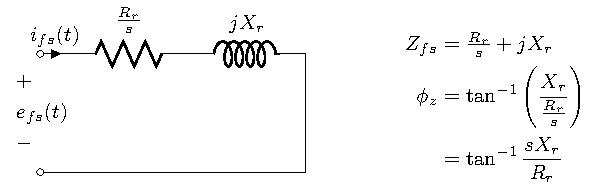
\includegraphics{figInductionRotorEquivalentStaticCircuit}
\begin{tikzpicture}
%grid
%\draw[gray] (-\sRo,-\sRo) grid (\sRo,\sRo);
\pgfmathsetmacro{\shiftX}{5cm}
\draw (0,0) to [short,o-,i={$i_{fs}(t)$}] ++(0.5,0) to [resistor,l={$\tfrac{R_r}{s}$}]++(2,0) to [inductor,l={$j X_{r}$}] ++(2,0) to ++(0,-2) to [short,-o] (0,-2);
\draw node at (0,-1){$\begin{aligned} &+\\ & e_{fs}(t)\\ &- \end{aligned}$};
\draw node[below right] at (6,0.5){$
\begin{aligned}
Z_{fs}&=\tfrac{R_r}{s}+j X_r\\
\phi_{fZ}&=\tan^{-1} \left( \frac{X_r}{\tfrac{R_r}{s}}\right)\\
&=\tan^{-1} \frac{s X_r}{R_r}
\end{aligned}$};
\end{tikzpicture}
\caption{گھومتے لچھوں کی جگہ فرضی ساکن لچھے کا دور۔}
\label{شکل_امالی_گھومتی_لچھوں_کا_فرضی_مساوی_ساکن_دور}
\end{figure}

مزید فرض کریں ان فرضی ساکن لچھوں کی مزاحمت \عددیء{\tfrac{R_r}{s}}  اور متعاملیت  \عددیء{j X_r} ہو:
\begin{align}
Z_{fs}=\frac{R_r}{s}+j X_r
\end{align}
اگر ان فرضی ساکن لچھوں پر مساوات \حوالہ{مساوات_امالی_تین_دباو}  کے برقی دباو لاگو کیے جائیں جیسا شکل \حوالہ{شکل_امالی_گھومتی_لچھوں_کا_فرضی_مساوی_ساکن_دور}  میں دکھایا گیا ہے تب ان میں درج ذیل برقی رو ہوں گے۔
\begin{gather}
\begin{aligned}
i_{afs}(t)&=\frac{E_r}{\sqrt{\left(\frac{R_r}{s} \right)^2+X_r^2}} \cos \left(\omega_e t+90\degree -\phi_Z  \right)=I_{or} \cos \left(\omega_e t+\theta_0 \right)\\
i_{bfs}(t)&=\frac{E_r}{\sqrt{\left(\frac{R_r}{s} \right)^2+X_r^2}} \cos \left(\omega_e t-30\degree -\phi_Z  \right)=I_{or}\cos \left(\omega_e t-120\degree +\theta_0 \right)\\
i_{cfs}(t)&=\frac{E_r}{\sqrt{\left(\frac{R_r}{s} \right)^2+X_r^2}} \cos \left(\omega_e t+210\degree -\phi_Z  \right)=I_{or} \cos \left(\omega_e t+120\degree+\theta_0 \right)
\end{aligned}
\end{gather}
مساوات \حوالہ{مساوات_امالی_گھومتا_رو}  \عددی{I_{0r}} اور \عددی{\theta_0} دیتی ہے۔دھیان رہے کہ ان مساوات میں  رکاوٹ کا زاویہ \عددیء{\phi_{fZ}}  وہی ہے جو گھومتے لچھے کا تھا:
\begin{align}
\phi_{fZ}=\tan^{-1} \frac{X}{\left(\frac{R}{s} \right)}=\tan^{-1} \frac{s X}{R}=\phi_Z
\end{align}
ان  رو کا تعدد \عددیء{\omega_e} اور پیدا کردہ گھومتا مقناطیسی موج درج ذیل ہو گا جو ہو بہو گھومتے لچھے کی موج \عددیء{\tau_{r,s}^+(\theta,t)} (مساوات \حوالہ{مساوات_امالی_گھومتے_حصے_کی_موج}) ہے۔
\begin{align}
\tau_{fs,s}^+(\theta,t)=k_w \frac{4}{\pi}\frac{N_r I_{0r}}{2} \cos (\theta-\omega_e t-\theta_0)
\end{align}

\حصہ{امالی موٹر کا مساوی برقی دور}
ہم ٹرانسفارمر کے ابتدائی لچھے کا برقی دور پہلے بنا چکے ہیں جہاں  لچھے کی مزاحمت \عددیء{R_1} اور  رستا متعاملیت\فرہنگ{رستا متعاملیت}\حاشیہب{leakage reactance}  \عددیء{j X_1} تھی۔ ٹرانسفارمر کے قالب  میں وقت کے ساتھ بدلتا مقناطیسی بہاو اس لچھے میں امالی برقی دباو \عددیء{\hat{E}_1} پیدا کرتا ہے۔ یوں 
\begin{align}
\hat{V}_1=\hat{I}_1 \left(R_1+j X_1 \right) +\hat{E}_1
\end{align}
لکھا جا سکتا ہے  جہاں \عددیء{\hat{V}_1} ابتدائی لچھے پر لاگو بیرونی برقی دباو ہے۔ہم دیکھیں گے کہ امالی موٹر کے ساکن لچھے کے لئے بھی یہی مساوات حاصل ہو گی۔
\begin{figure}
\centering
%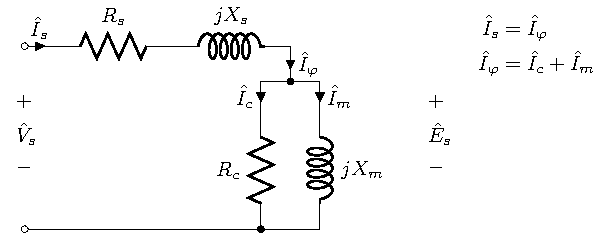
\includegraphics{figInductionStatorEquivalentCircuit}
\begin{tikzpicture}
%grid
%\draw[gray] (-\sRo,-\sRo) grid (\sRo,\sRo);
\pgfmathsetmacro{\shiftX}{5cm}
\draw (0,0) to [short,o-,i={$\hat{I}_s $}] ++(0.5,0) to [resistor,l={$R_s$}]++(2,0) to [inductor,l={$j X_{s}$}] ++(2,0) to [short,-*,i={$\hat{I}_\varphi$}] ++(0,-0.6)coordinate(upperJunction) to [short] ++(-0.5,0) to [short,i_={$\hat{I}_c$}] ++(0,-0.5) to  [resistor,l_={$R_c$}] ++(0,-2) to [short,-o] ++(-4,0)coordinate(lowerLeftTerminal);
\draw (upperJunction) to [short] ++(0.5,0) to [short,i={$\hat{I}_m$}] ++(0,-0.5) to  [inductor,l={$jX_m$}] ++(0,-2) to [short,-*] ++(-1,0);
%
\draw node at (0,-1.5){$\begin{aligned} &+\\ & \hat{V}_s\\ &- \end{aligned}$};
\draw node at (7,-2.125){$\begin{aligned} &+\\ & \hat{E}_s\\ &- \end{aligned}$};
\draw node[right] at (7.5,0){$\begin{aligned}  \hat{I}_s&=\hat{I}_\varphi\\ \hat{I}_\varphi&=\hat{I}_c+\hat{I}_m \end{aligned}$};
\end{tikzpicture}
\caption{امالی موٹر کے ساکن لچھوں کا مساوی برقی دور۔}
\label{شکل_امالی_ساکن_لچھوں_کی_مساوی_دور}
\end{figure}

 تصور کریں کہ مشین کے گھومتے لچھے کھلا دور ہیں اور  ساکن لچھوں پر تین دوری برقی دباو لاگو ہے۔ ساکن لچھوں کے برقی رو  گھومتے مقناطیسی دباو کی ایک موج \عددیء{\tau_{s}^+(\theta,t)}  پیدا کریں گے جو مساوات \حوالہ{مساوات_امالی_گھومتا_مقناطیسی_دباو_الف} میں دی گئی ہے۔

اس حصہ میں ہم مشین کے ایک دور، مثلاً دور \عددیء{a}،  پر نظر رکھیں گے۔ یہاں شکل  \حوالہ{شکل_امالی_ساکن_لچھوں_کی_مساوی_دور} سے رجوع کریں۔اگر ساکن لچھے کی مزاحمت \عددیء{R_s} اور متعاملیت \عددیء{j X_s} ہو اور اس پر لاگو بیرونی برقی دباو \عددیء{v_s(t)} ہو تب \اصطلاح{کرخوف}\حاشیہب{Kirchoff's voltage law} کے برقی دباو کے قانون کے تحت درج ذیل ہو گا
\begin{align}
v_s(t)=i_s R_s +L_s \frac{\dif i_s}{\dif t}+e_s(t)
\end{align}
جہاں \عددیء{e_s(t) }،  مساوات \حوالہ{مساوات_امالی_تین_دور_سائن_نما_برقی_دباو}  میں دی گئی، اس موج کی ساکن لچھے میں پیدا امالی برقی دباو ہے ۔اسی کو دوری سمتیہ کی صورت میں لکھتے ہیں۔
\begin{align}\label{مساوات_امالی_دوری_موٹر_مساوات}
\hat{V}_s=\hat{I}_s \left(R_s+j X_s \right)+\hat{E}_s
\end{align}
ٹرانسفارمر کی مثال آگے بڑھاتے ہیں۔اگر موٹر کا گھومتا لچھا کھلا دور\حاشیہب{open circuited} رکھا جائے تب قالب میں ایک ہی گھومتے مقناطیسی دباو کی موج \عددیء{\tau_s^+(\theta,t)} ہو گی۔صرف ساکن لچھے میں برقی رو (\عددیء{\hat{I}_\varphi}) ہو گا جو قالب میں مقناطیسی بہاو \عددیء{\varphi_s} پیدا کرے گا۔ یہ برقی رو \عددیء{\hat{I}_\varphi} غیر سائن نما ہو گا۔ \اصطلاح{فوریئر} تسلسل\حاشیہب{Fourier series} کی مدد سے اس کے بنیادی  اور ہارمونی اجزاء دریافت کئے جا سکتے ہیں۔ اس کے بنیادی جزو کے دو حصے ہوں گے۔ ایک حصہ  \عددیء{\hat{I}_c}، لاگو بیرونی برقی دباو \عددیء{\hat{V}_s} کے ہم قدم اور قالب میں طاقت کے ضیاع کو ظاہر کرے گا جبکہ  دوسرا حصہ \عددیء{\hat{V}_s} سے نوے درجہ تاخیری زاویہ پر ہو گا۔\عددیء{\hat{I}_\varphi}میں سے \عددیء{\hat{I}_c} منفی کر کے \اصطلاح{ مقناطیسی جزو} حاصل ہو گا جس کو  \عددیء{\hat{I}_m} سے ظاہر کیا جاتا ہے۔ بنیادی جزو کے لحاظ سے مقناطیسی جزو  تاخیری   اور باقی سارے ہارمونی اجزاء کا مجموعہ ہو گا
\begin{align}
\hat{I}_\varphi=\hat{I}_c+\hat{I}_m
\end{align}
جو قالب میں مقناطیسی بہاو \عددیء{\varphi_s} پیدا کرتا ہے۔ امالی موٹر کے مساوی دور میں \عددیء{\hat{I}_c} کو مزاحمت \عددیء{R_c} سے اور \عددیء{\hat{I}_m} کو \عددیء{j X_\varphi} سے یوں ظاہر کیا جاتا ہے کہ چلتی موٹر میں، متوقع برقی تعدد  اور امالی برقی دباو \عددیء{\hat{E}_s} پر،  \عددی{R_c} میں \عددی{I_c} اور \عددی{X_m} میں \عددی{I_m} برقی رو حاصل ہو۔یوں درج ذیل ہو گا۔
\begin{gather}
\begin{aligned}
R_c&=\frac{\hat{E}_s}{\hat{I}_c}=\frac{E_s}{I_c}\\
X_\varphi&=\frac{\abs{\hat{E}_s}}{\abs{\hat{I}_m}}=\frac{E_s}{I_m}
\end{aligned}
\end{gather}
مقناطیسی دباو کی موج \عددیء{\tau_s^+(\theta,t)} گھومتے لچھے میں بھی امالی برقی دباو پیدا کرے گی۔مساوات \حوالہ{مساوات_امالی_دوری_موٹر_مساوات}  میں  اگر رکاوٹ میں برقی دباو کے گھٹنے کو نظر انداز کیا جائے تب لاگو بیرونی برقی دباو اور لچھے کا اندرونی امالی برقی دباو ہر حالت میں ایک دوسرے کے برابر ہوں گے۔اب تصور کریں کہ گھومتے لچھے کسر دور کر دیے جاتے ہیں۔ ایسا کرتے ہی ان میں برقی رو گزرنے لگے گیں جو مقناطیسی دباو کی موج  \عددیء{\tau_{r,s}^+(\theta,t)}، جو مساوات \حوالہ{مساوات_امالی_گھومتے_حصے_کی_موج}  میں دی گئی ہے،  پیدا کریں گے۔ اس موج سے ساکن لچھے میں امالی برقی دباو \عددیء{\hat{E}_s} تبدیل ہو  گا لہٰذا امالی برقی دباو اور  لاگو برقی دباو ایک دوسرے کے برابر نہیں رہیں گے۔ یہ ایک نا ممکنہ صورت حال ہے۔

ساکن لچھے میں امالی برقی دباو،  لاگو برقی دباو کے برابر تب رہے گا جب قالب میں مقناطیسی دباو تبدیل نہ ہو۔ مشین کے قالب میں مقناطیسی دباو برقرار یوں رہتا ہے کہ ساکن لچھے،  مقناطیسی دباو \عددیء{\tau_{r,s}^+(\theta,t)}  کی متضاد، مقناطیسی دباو کی ایک موج پیدا کرتے ہیں جو \عددیء{\tau_{r,s}^+(\theta,t)} کے اثر کو مکمل طور پر ختم کر دیتی ہے۔یہ موج پیدا کرنے کے لئے ساکن لچھوں میں برقی رو \عددیء{\hat{I}_\varphi} سے بڑھ کر \عددیء{(\hat{I}_\varphi+\hat{I}_r')} ہو جاتے ہیں جہاں اضافی برقی رو درج ذیل ہوں  گے۔
\begin{gather}
\begin{aligned}\label{مساوات_امالی_تین_رو_الف}
i_{ar}'(t)&=I_{or}' \cos (\omega_e t+\theta_0)\\
i_{br}'(t)&=I_{or}' \cos (\omega_e t-120\degree+\theta_0)\\
i_{cr}'(t)&=I_{or}' \cos (\omega_e t+120\degree+\theta_0)
\end{aligned}
\end{gather}
یہ اضافی برقی رو درج ذیل موج پیدا کرتے ہیں۔
\begin{align}\label{مساوات_امالی_اضافی_موج}
\tau_{(r)}^+(\theta,t)=k_w \frac{4}{\pi}\frac{N_s I_{0r}'}{2} \cos (\theta-\omega_e t -\theta_0)
\end{align}
ساکن لچھوں میں اضافی برقی رو نے ہر لمحہ گھومتے لچھوں کے برقی رو کے اثر کو ختم کرنا ہے لہٰذا یہ دونوں برقی رو ہم قدم\حاشیہب{in-phase}  ہوں گے۔چونکہ  مساوات \حوالہ{مساوات_امالی_اضافی_موج} اور مساوات \حوالہ{مساوات_امالی_گھومتے_حصے_کی_موج} ہر لمحہ ایک دوسرے کے  برابر ہیں لہٰذا درج ذیل ہو گا۔
\begin{align}
N_s I_{0r}'=N_r I_{0r}
\end{align}
مساوات \حوالہ{مساوات_امالی_گھومتا_رو} کی استعمال سے  درج ذیل ہو گا۔
\begin{align}
I_{0r}'&=\left(\frac{N_r}{N_s}\right) I_{0r}=\left(\frac{N_r}{N_s}\right) \frac{s E_r}{\sqrt{R_r^2+s^2 X_r^2}}
\end{align}
آپ نے دیکھا کہ گھومتے لچھے مقناطیسی دباو کی موج پیدا کرتے ہیں جن کے ذریعہ ساکن لچھوں کو معلوم ہوتا ہے کہ موٹر پر بوجھ لدا ہے اور وہ اس کے مطابق لاگو برقی دباو سے برقی رو لیتی ہیں۔یہاں تک امالی موٹر کا مساوی برقی دور شکل \حوالہ{شکل_امالی_ساکن_کا_مساوی_دور_بمع_گھومتے_لچھے_کی_رو}  میں دکھایا گیا ہے۔
\begin{figure}
\centering
%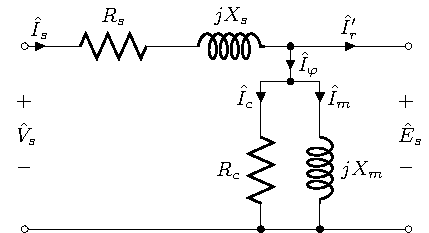
\includegraphics{figInductionStatorEquivalentCircuitWithRotorCurrent}
\begin{tikzpicture}
%grid
%\draw[gray] (-\sRo,-\sRo) grid (\sRo,\sRo);
\pgfmathsetmacro{\shiftX}{5cm}
\draw (0,0) to [short,o-,i={$\hat{I}_s $}] ++(0.5,0) to [resistor,l={$R_s$}]++(2,0) to [inductor,l={$j X_{s}$}] ++(2,0)coordinate(rotorStartUp) to [short,-*,i={$\hat{I}_\varphi$}] ++(0,-0.6)coordinate(upperJunction) to [short] ++(-0.5,0) to [short,i_={$\hat{I}_c$}] ++(0,-0.5) to  [resistor,l_={$R_c$}] ++(0,-2) to [short,-o] ++(-4,0)coordinate(lowerLeftTerminal);
\draw (upperJunction) to [short] ++(0.5,0) to [short,i={$\hat{I}_m$}] ++(0,-0.5) to  [inductor,l={$jX_m$}] ++(0,-2)coordinate(rotorStartLow) to [short,-*] ++(-1,0);
\draw (rotorStartUp) to [short,*-o,i={$\hat{I}_r'$}] ++(2,0);
\draw (rotorStartLow) to [short,*-o] ++(1.5,0);
%
\draw node at (0,-1.5){$\begin{aligned} &+\\ & \hat{V}_s\\ &- \end{aligned}$};
\draw node at (6.5,-1.5){$\begin{aligned} &+\\ & \hat{E}_s\\ &- \end{aligned}$};
\end{tikzpicture}
\caption{مساوی دور اضافی برقی رو کے ساتھ۔}
\label{شکل_امالی_ساکن_کا_مساوی_دور_بمع_گھومتے_لچھے_کی_رو}
\end{figure}
%
\begin{figure}
\centering
%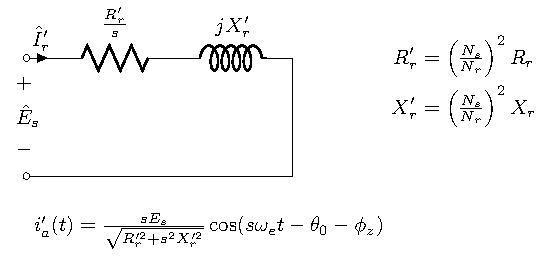
\includegraphics{figInductionRotorEquivalentAnotherCircuit}
\begin{tikzpicture}
%grid
%\draw[gray] (-\sRo,-\sRo) grid (\sRo,\sRo);
\pgfmathsetmacro{\shiftX}{5cm}
\draw (0,0) to [short,o-,i={$\hat{I}_r'$}] ++(0.5,0) to [resistor,l={$\tfrac{R_r'}{s}$}]++(2,0) to [inductor,l={$jX_{r}'$}] ++(2,0) to ++(0,-2) to [short,-o] (0,-2);
\draw node at (0,-1){$\begin{aligned} &+\\ & \hat{E}_s\\ &- \end{aligned}$};
\draw node[below right] at (6,0.5){$
\begin{aligned}
R_r'&=\left(\tfrac{N_s}{N_r} \right)^2 R_r\\
X_r'&=\left(\tfrac{N_s}{N_r} \right)^2 X_r
\end{aligned}$};
%
\draw node[below right] at (0,-2.5){$
i_a'(t)=\tfrac{s E_s}{\sqrt{R_r'^2+s^2X_r'^2}} \cos (\omega_e t -\theta_0-\phi_z)  $}; 
\end{tikzpicture}
\caption{گھومتے لچھے کا ایک  مساوی دور۔}
\label{شکل_امالی_گھومتے_لچھے_کا_دوسرا_مساوی_دور}
\end{figure}
یہاں ذرہ شکل \حوالہ{شکل_امالی_گھومتے_لچھے_کا_دوسرا_مساوی_دور}  سے رجوع کریں جہاں 
\begin{gather}
\begin{aligned}\label{مساوات_امالی_گھومتے_مزاحمت_امالہ_دوسری_جانب}
R_r'&=\left(\frac{N_s}{N_r} \right)^2 R_r\\
X_r'&=\left(\frac{N_s}{N_r} \right)^2 X_r
\end{aligned}
\end{gather} 
پر ساکن لچھوں کا امالی برقی دباو \عددیء{\hat{E}_s} لاگو ہے لہٰذا  برقی رو درج ذیل ہوں گے۔
\begin{gather}
\begin{aligned}\label{مساوات_امالی_تین_رو}
i_a'(t)&=\frac{s E_s}{\sqrt{R_r'^2+s^2 X_r'^2}} \cos (\omega_e t +90\degree -\phi_Z)\\
i_b'(t)&=\frac{s E_s}{\sqrt{R_r'^2+s^2 X_r'^2}} \cos (\omega_e t -30\degree -\phi_Z)\\
i_c'(t)&=\frac{s E_s}{\sqrt{R_r'^2+s^2 X_r'^2}} \cos (\omega_e t +210\degree -\phi_Z)
\end{aligned}
\end{gather}
ان سب  کے حیطے ایک دوسرے کے برابر ہیں۔اس حیطہ کو 
\begin{align}\label{مساوات_امالی_رو_دباو_تعلق_الف}
\frac{s E_s}{\sqrt{R_r'^2+s^2 X_r'^2}}=\frac{s \omega_e N_s \phi_0}{\sqrt{\left( \frac{N_s}{N_r}\right)^2 \left(R_r^2+s^2X_r^2 \right)}}=\left(\frac{N_r}{N_s}\right) I_{0r}=I_{0r}'
\end{align}
لکھ کر  مساوات \حوالہ{مساوات_امالی_تین_رو}  کو درج ذیل صورت میں لکھا جا سکتا ہے۔
\begin{gather}
\begin{aligned}
i_a'(t)&=I_{0r}' \cos (\omega_e t +90\degree -\phi_Z)\\
i_b'(t)&=I_{0r}' \cos (\omega_e t -30\degree -\phi_Z)\\
i_c'(t)&=I_{0r}' \cos (\omega_e t +210\degree -\phi_Z)
\end{aligned}
\end{gather}
یہ مساوات بالکل مساوات \حوالہ{مساوات_امالی_تین_رو_الف}  کی طرح ہے جہاں \عددی{\theta_0=90-\phi_Z} ہو گا۔ یوں شکل \حوالہ{شکل_امالی_ساکن_کا_مساوی_دور_بمع_گھومتے_لچھے_کی_رو}  میں ساکن لچھوں کے امالی برقی دباو \عددیء{\hat{E}_s} کے متوازی شکل \حوالہ{شکل_امالی_گھومتے_لچھے_کا_دوسرا_مساوی_دور}  جوڑنے سے ساکن لچھوں میں  اضافی برقی رو  اتنا ہی ہو گا جتنا اصل موٹر میں گھومتے لچھوں کی بنا ہو گا۔ ایسا کرتے ہوئے شکل \حوالہ{شکل_امالی_مشین_کا_مکمل_مساوی_دور}  حاصل ہوتی ہے جو امالی موٹر کا مساوی برقی دور ہے اور  جو امالی موٹر  کی صحیح عکاسی کرتا ہے۔
\begin{figure}
\centering
%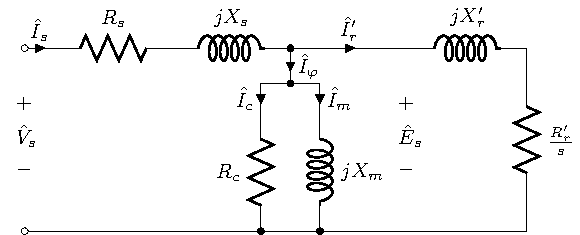
\includegraphics{figInductionMachineEquivalentCircuit}
\begin{tikzpicture}
%grid
%\draw[gray] (-\sRo,-\sRo) grid (\sRo,\sRo);
\pgfmathsetmacro{\shiftX}{5cm}
\draw (0,0) to [short,o-,i={$\hat{I}_s $}] ++(0.5,0) to [resistor,l={$R_s$}]++(2,0) to [inductor,l={$j X_{s}$}] ++(2,0)coordinate(rotorStartUp) to [short,-*,i={$\hat{I}_\varphi$}] ++(0,-0.6)coordinate(upperJunction) to [short] ++(-0.5,0) to [short,i_={$\hat{I}_c$}] ++(0,-0.5) to  [resistor,l_={$R_c$}] ++(0,-2) to [short,-o] ++(-4,0)coordinate(lowerLeftTerminal);
\draw (upperJunction) to [short] ++(0.5,0) to [short,i={$\hat{I}_m$}] ++(0,-0.5) to  [inductor,l={$j X_m$}] ++(0,-2)coordinate(rotorStartLow) to [short,-*] ++(-1,0);
\draw (rotorStartUp) to [short,*-,i={$\hat{I}_r'$}] ++(2,0) to [inductor,l={$j X_r'$}] ++(2,0) to [resistor,l={$\tfrac{R_r'}{s}$}] ++(0,-3.1) to [short] ++(-2,0);
\draw (rotorStartLow) to [short,*-] ++(1.5,0);
%
\draw node at (0,-1.5){$\begin{aligned} &+\\ & \hat{V}_s\\ &- \end{aligned}$};
\draw node at (6.5,-1.5){$\begin{aligned} &+\\ & \hat{E}_s\\ &- \end{aligned}$};
\end{tikzpicture}
\caption{امالی موٹر کا مساوی برقی دور۔}
\label{شکل_امالی_مشین_کا_مکمل_مساوی_دور}
\end{figure}


\حصہ{مساوی برقی دور پر غور}
ایک گھومتے لچھے میں برقی طاقت کے ضیاع کو مساوات \حوالہ{مساوات_امالی_طاقت_ضیاع_گھمتا_حصہ} ظاہر کرتی ہے۔مساوات \حوالہ{مساوات_امالی_گھومتے_مزاحمت_امالہ_دوسری_جانب}  اور \حوالہ{مساوات_امالی_رو_دباو_تعلق_الف}   کی مدد سے اسے درج ذیل  لکھا جا سکتا ہے۔
\begin{align}
p_{\textup{ضیاع}}&=I_{0r}^2 R_r=\left(\frac{N_s^2}{N_r^2} I_{0r}'^2 \right) \left (\frac{N_r^2}{N_s^2} R_r' \right)=I_{0r}'^2 R_r'
\end{align}
ہم  شکل \حوالہ{شکل_امالی_مشین_کا_مکمل_مساوی_دور} میں برقی دباو اور برقی رو  کی قیمتوں کو موثر قیمتیں تصور کرتے ہیں۔ یوں شکل \حوالہ{شکل_امالی_مشین_کا_مکمل_مساوی_دور} میں  گھومتے لچھے کو کل
\begin{align}\label{مساوات_امالی_میکانی_طاقت_بالمقابل_سرک_الف}
p_r = I_{0r}'^2 \frac{R_r'}{s}
\end{align}
برقی طاقت فراہم کی جائے گی جس میں سے \عددیء{p_{\textup{ضیاع}}} گھومتے لچھے کی مزاحمت میں ضائع ہو گی اور باقی بطور میکانی طاقت  مشین کے دھرے پر دستیاب ہو گی:
\begin{align}
p=I_{0r}'^2 \frac{R_r'}{s}-I_{0r}'^2 R_r'=I_{0r}'^2 \frac{R_r'}{s} (1-s)=p_r (1-s)
\end{align}
تین دوری مشین جس میں تین لچھے ہوتے ہیں تین گنا میکانی طاقت فراہم کرے گی:
\begin{align}\label{مساوات_امالی_تین_دور_میکانی_طاقت_بالمقابل_سرک_الف}
p_{\textup{میکانی}} =3 I_{0r}'^2 \frac{R_r'}{s} (1-s)=3 p_r (1-s)
\end{align}
 مساوات \حوالہ{مساوات_امالی_تین_دور_میکانی_طاقت_بالمقابل_سرک_الف} کہتی ہے کہ ساکن موٹر، جس کا سرکاو اکائی ہو گا، کوئی میکانی طاقت فراہم نہیں کرتی ہے بلکہ  وہ تمام برقی توانائی جو  گھومتے حصہ کو ملتی ہے ضائع ہو کر اس حصہ کو گرم کرتی ہے جس سے موٹر جلنے کا امکان ہوتا ہے۔ آپ اس مساوات سے دیکھ سکتے ہیں کہ امالی موٹر کا سرکاو صفر کے قریب رہنا چاہئے ورنہ یہ ناقابل قبول (اور ناقابل برداشت) حد تک برقی توانائی ضائع کرے گی۔ ہم امالی موٹر کی مساوی برقی دور کو شکل \حوالہ{شکل_امالی_مشین_کا_دوسرا_مکمل_مساوی_دور}  کی طرح بھی تشکیل دے  سکتے ہیں جس  میں شکل \حوالہ{شکل_امالی_مشین_کا_مکمل_مساوی_دور}  کی مزاحمت  \عددیء{\tfrac{R_r'}{s}} کو دو حصوں میں تقسیم کیا گیا ہے:
\begin{align*}
\frac{R_r'}{s}=R_r'+ R_r' \left( \frac{1-s} {s}\right)
\end{align*}
یوں شکل \حوالہ{شکل_امالی_مشین_کا_مکمل_مساوی_دور}  میں مزاحمت  \عددیء{R_r'} میں برقی طاقت کا ضیاع \عددیء{I_{0r}'^2 R_r'} گھومتے لچھے کا ضیاع جبکہ مزاحمت \عددیء{R_r' \left(\tfrac{1-s}{s} \right)} میں برقی طاقت کا ضیاع \عددیء{I_{0r}'^2 R_r' \left(\tfrac{1-s}{s} \right)} دراصل میکانی طاقت  ہو گا۔یاد رہے کہ تین دوری  مشین کے لئے ان نتائج کو تین سے ضرب دینا ہو گا۔
\begin{figure}
\centering
%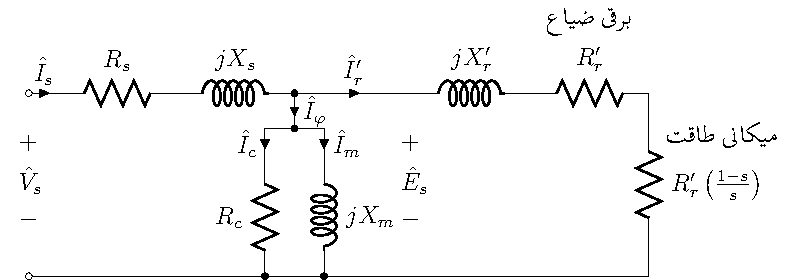
\includegraphics{figInductionMachineAnotherEquivalentCircuit}
\begin{tikzpicture}
\draw (0,0) to [short,o-,i={$\hat{I}_s $}] ++(0.5,0) to [resistor,l={$R_s$}]++(2,0) to [inductor,l={$j X_{s}$}] ++(2,0)coordinate(rotorStartUp) to [short,-*,i={$\hat{I}_\varphi$}] ++(0,-0.6)coordinate(upperJunction) to [short] ++(-0.5,0) to [short,i_={$\hat{I}_c$}] ++(0,-0.5) to  [resistor,l_={$R_c$}] ++(0,-2) to [short,-o] ++(-4,0)coordinate(lowerLeftTerminal);
\draw (upperJunction) to [short] ++(0.5,0) to [short,i={$\hat{I}_m$}] ++(0,-0.5) to  [inductor,l={$jX_m$}] ++(0,-2)coordinate(rotorStartLow) to [short,-*] ++(-1,0);
\draw (rotorStartUp) to [short,*-,i={$\hat{I}_r'$}] ++(2,0) to [inductor,l={$j X_r'$}] ++(2,0) to [resistor,l={$R_r'$}] ++(2,0) to [resistor,l={$R_r' \left( \tfrac{1-s}{s}\right)$}] ++(0,-3.1) to [short] ++(-4,0);
\draw (rotorStartLow) to [short,*-] ++(1.5,0);
%text
\node at (9.5,1.2){\RL{برقی ضیاع}};
\node at (11.75,-0.7){\RL{میکانی طاقت}};
%
\draw node at (0,-1.5){$\begin{aligned} &+\\ & \hat{V}_s\\ &- \end{aligned}$};
\draw node at (6.5,-1.5){$\begin{aligned} &+\\ & \hat{E}_s\\ &- \end{aligned}$};
\end{tikzpicture}
\caption{امالی موٹر کا دوسرا مساوی برقی دور۔}
\label{شکل_امالی_مشین_کا_دوسرا_مکمل_مساوی_دور}
\end{figure}

میکانی طاقت سے مراد  قوت مروڑ ضرب میکانی زاویائی رفتار  ہے۔ امالی موٹر کی میکانی زاویائی رفتار مساوات \حوالہ{مساوات_امالی_سرک_اور_تعدد}  دیتی ہے جبکہ مساوات \حوالہ{مساوات_گھومتے_مشین_برقی_میکانی_رفتار_تعلق}  میں میکانی معاصر رفتار \عددیء{\omega_{sm}} دیتی ہے۔یوں میکانی طاقت
\begin{align}\label{مساوات_امالی_تین_دور_میکانی_طاقت_اور_رفتار}
p= T_m \omega =T_m \times 2 \pi f=T_m \times 2 \pi (1-s) f_s=T_m (1-s) \omega_{sm} 
\end{align}
اور قوت مروڑ درج ذیل ہو گی۔
\begin{align}\label{مساوات_امالی_مروڑ_الف}
T_m=\frac{p}{(1-s) \omega_{sm}}=\frac{3 I_{0r}'^2}{\omega_{sm}} \frac{R_r'}{s}
\end{align}
اصل موٹر میں رگڑ، قالبی ضیاع، لچھوں میں ضیاع اور دیگر وجوہات کی بنا، دھرے پر طاقت یا قوت مروڑ ان سے  کم ہو گی۔

ٹرانسفارمر کے سادہ ترین مساوی دور میں \عددیء{R_c} اور \عددیء{X_m} کو نظرانداز کیا گیا تھا۔ امالی موٹر میں ایسا کرنا ممکن نہیں ہوتا چونکہ موٹروں میں خلائی درز ہوتی ہے جس میں مقناطیسی بہاو پیدا کرنے کے لئے بہت زیادہ مقناطیسی دباو درکار ہوتی ہے۔بے بوجھ امالی موٹر کو بناوٹی برقی رو کا تیس سے پچاس فی صد برقی رو، قالب کو ہیجان کرنے کے لئے درکار ہوتا ہے۔ مزید، خلائی درز کی وجہ سے اس کی رستا امالہ بھی زیادہ ہوتا ہے اور اسے نظر انداز کرنا ممکن نہیں ہوتا۔ البتہ مساوی دور میں \عددیء{R_c} کو نظرانداز کیا جا سکتا ہے جیسے شکل \حوالہ{شکل_امالی_ساکن_حصے_کا_تھونن_دور} میں کیا گیا ہے۔ اس شکل میں نقطہ دار لکیر کی بائیں جانب کا مساوی تھونن دور بنایا جا سکتا ہے۔ایسا کرنے سے امالی موٹر پر غور کرنا  آسان ہو جاتا ہے۔ اب ہم ایسا ہی کرتے ہیں۔
\begin{figure}
\centering
%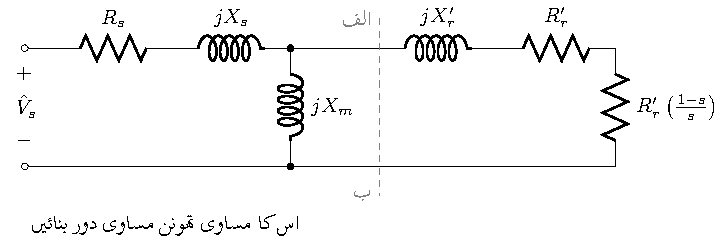
\includegraphics{figInductionMachineTheveninNeededOfStatorSide}
\begin{tikzpicture}
%grid
%\draw[gray] (-\sRo,-\sRo) grid (\sRo,\sRo);
%
\draw (0,0) to [short,o-] ++(0.5,0) to [resistor,l={$R_s$}]++(2,0) to [inductor,l={$j X_{s}$}] ++(2,0)coordinate(rotorStartUp) to [inductor,*-,l={$j X_m$}] ++(0,-2)coordinate(statorLowerRight) to [short,-o](0,-2);
\draw (rotorStartUp)  to ++(1.5,0) to [inductor,l={$j X_r'$}] ++(2,0) to [resistor,l={$R_r'$}] ++(2,0) to [resistor,l={$R_r' \left( \tfrac{1-s}{s}\right)$}] ++(0,-2) to [short,-*] (statorLowerRight);
%text
\draw node[below right] at (1,-2){\RL{اس حصہ کا مساوی تھونن دور بنائیں}};
\draw[dashed] (rotorStartUp)++(1.5,0.5)node[left]{ا}--++(0,-3)node[left]{ب};
%text
%
\draw node at (0,-1){$\begin{aligned} &+\\ & \hat{V}_s\\ &- \end{aligned}$};
\end{tikzpicture}
\caption{امالی موٹر کا سادہ دور۔ قالبی ضیاع کو نظرانداز کیا گیا ہے۔}
\label{شکل_امالی_ساکن_حصے_کا_تھونن_دور}
\end{figure}
%
\ابتدا{مثال}\شناخت{مثال_امالی_ستارہ_چھ_قطب_پندرہ_کلو_واٹ}
ستارہ، چھ قطبی، پچاس ہرٹز اور  \عددیء{415} وولٹ پر چلنے والی  \عددیء{15} کلو واٹ امالی موٹر کے مساوی دور کے اجزاء درج ذیل ہیں۔
\begin{align*}
R_s= \SI{0.5}{\ohm}, \quad R_r'=\SI{0.31}{\ohm}, \quad X_s=\SI{0.9}{\ohm}, \quad X_r'=\SI{0.34}{\ohm}, \quad X_m=\SI{0.22}{\ohm} 
\end{align*}
موٹر میں رگڑ سے طاقت کا ضیاع  \عددیء{600} واٹ ہے۔قالبی ضیاع کو اسی کا حصہ تصور کیا گیا ہے۔ اس کو اٹل تصور کیا جائے۔یہ موٹر درکار وولٹ اور تعداد  پر دو فی صد سرکاو پر چل رہی ہے۔اس حالت میں موٹر کی رفتار، اس کے دھرے پر پیدا قوت مروڑ اور طاقت، اس کے ساکن لچھے کا برقی رو اور اس کی فی صد کارگزاری حاصل کریں۔

حل:\quad
موٹر کی معاصر رفتار \عددیء{f_m=\tfrac{2}{6} \times 50=16.66} چکر فی سیکنڈ یا \عددیء{16.66\times 60=1000} چکر فی منٹ ہو گی۔دو فی صد سرکاو پر موٹر کی رفتار \عددیء{f=16.66 \times (1-0.02)=16.33} چکر فی سیکنڈ یا  \عددیء{16.33 \times 60=979.8} چکر فی منٹ ہو گی۔

شکل \حوالہ{شکل_امالی_ساکن_حصے_کا_تھونن_دور}  میں دائیں جانب
\begin{align*}
j X_r'+R_r'+R_r' \frac{1-s}{s}=j X_r'+\frac{R_r'}{s}=j 0.34+\frac{0.31}{0.02}=j 0.34+15.5
\end{align*}
اور \عددیء{j X_m} متوازی جڑے ہیں جن کی مساوی رکاوٹ درج ذیل ہو گی۔
\begin{align*}
\frac{1}{Z}&=\frac{1}{15.5+j 0.34}+\frac{1}{j 22}\\
Z&=10.147+j 7.375=R+jX
\end{align*}
موٹر پر لاگو  یک دوری برقی دباو  \عددیء{\tfrac{415}{\sqrt{3}}=239.6} وولٹ ہے۔ یوں ساکن لچھے کا برقی رو درج ذیل ہو گا۔
\begin{align*}
\hat{I}_s&=\frac{\hat{V}_s}{R_s+j X_s+Z}\\
&=\frac{239.6}{0.5+j0.99+10.147+j 7.375}\\
&=17.6956 \phase{-38.155 \degree}
\end{align*}
اس موٹر کے گھومتے حصہ کو وہی طاقت منتقل ہو گی جو رکاوٹ \عددیء{Z}  کو منتقل ہو گی۔یوں مساوات \حوالہ{مساوات_امالی_میکانی_طاقت_بالمقابل_سرک_الف}  درج ذیل لکھی جا سکتی ہے۔
\begin{align*}
p=I_{or}'^2 \frac{R_r'}{s}=I_s^2 R=17.6956^2 \times 10.147=\SI{3177.37}{\watt}
\end{align*}
تین دور کے لئے   \عددیء{3 \times 3177.37=9532} واٹ ہو گی۔مساوات \حوالہ{مساوات_امالی_تین_دور_میکانی_طاقت_بالمقابل_سرک_الف}  موٹر کی اندرونی میکانی طاقت دیتی ہے:
\begin{align*}
p_{\textup{میکانی}}=
9532 \times (1-0.02)=\SI{9341}{\watt}
\end{align*}
اس سے طاقت کا ضیاع منفی کرنے سے  موٹر کے دھرے پر میکانی طاقت \عددیء{9341-600=8741} واٹ حاصل ہوتی ہے لہٰذا دھرے پر قوت مروڑ درج ذیل ہو گی۔
\begin{align*}
T=\frac{8741}{2 \times \pi \times 16.33}=\SI{85.1}{\newton \meter}
\end{align*}

موٹر کو کل مہیا برقی طاقت \عددیء{\sqrt{3} \times 415 \times 17.6956 \times \cos (-38.155)=10001.97} واٹ ہو گی۔ یوں اس موٹر کی کارگزاری  \عددیء{\tfrac{8741}{10001.97} \times 100=\SI{87.39}{\percent}} ہو گی۔
\انتہا{مثال}
%
\حصہ{امالی موٹر کا مساوی تھونن دور  یا ریاضی نمونہ}
مسئلہ \اصطلاح{تھونن}\فرہنگ{مسئلہ!تھونن}\حاشیہب{Thevenin theorem}\فرہنگ{Thevenin theorem} کے مطابق کسی بھی سادہ خطی برقی دور\فرہنگ{خطی!برقی دور}\حاشیہب{linear circuit}\فرہنگ{linear circuit} کو اس کے دو برقی سروں کے مابین ایک رکاوٹ اور ایک برقی دباو کی مساوی سلسلہ وار دور سے ظاہر کیا جا سکتا ہے۔اس مساوی دور کو مساوی تھونن دور کہتے ہیں جبکہ اس مساوی تھونن دور کی رکاوٹ کو تھونن رکاوٹ اور برقی دباو کو تھونن برقی دباو کہتے ہیں۔

برقی دور کے دو برقی سروں کے بیچ تھونن رکاوٹ حاصل کرنے کے لئے  برقی دور کے تمام اندرونی برقی دباو کسر دور کر کے ان دو برقی سروں کے بیچ رکاوٹ معلوم کی جاتی ہے۔یہی رکاوٹ، تھونن رکاوٹ ہو گی۔انہیں برقی سروں پر تھونن برقی دباو حاصل کرنے کے لئے دیے گئے برقی دور کے تمام اندرونی برقی دباو برقرار رکھ کر ان دو سروں پر برقی دباو معلوم کیا جاتا ہے۔ یہی برقی دباو در حقیقت تھونن برقی دباو ہو گا۔بعض اوقات ہم ایک برقی دور کے ایک خاص حصے کا مساوی تھوِنن دور بنانا چاہتے ہیں۔ایسا کرتے وقت باقی برقی دور کو اس حصے سے مکمل طور پر منقطع کر کے درکار حصہ کا تھونن مساوی دور حاصل کیا جاتا ہے۔
\begin{figure}
\centering
%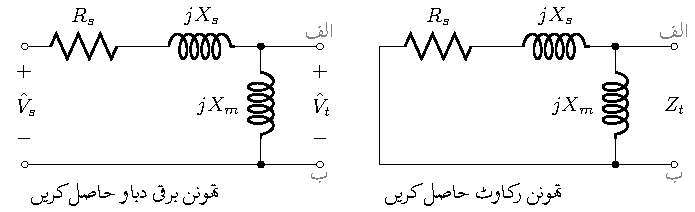
\includegraphics{figInductionMachineTheveninImpedanceAndVoltage}
\begin{subfigure}{0.45\textwidth}
\centering
\begin{tikzpicture}
\draw (0,0)  to [resistor,l={$R_s$}]++(2,0) to [inductor,l={$j X_{s}$}] ++(2,0)coordinate(rotorStartUp) to [inductor,l_={$j X_m$}] ++(0,-2)coordinate(statorLowerRight) to (0,-2) to (0,0);
\draw(rotorStartUp) to [short,*-o] ++(1,0)node[above]{ا};
\draw(statorLowerRight) to [short,*-o] ++(1,0)node[below]{ب};
%text
\draw node[right] at (0,-2.5){\RL{تھونن رکاوٹ حاصل کریں}};
\draw node at (5,-1){$Z_{t}$};
\end{tikzpicture}
\end{subfigure}\hfill
\begin{subfigure}{0.45\textwidth}
\centering
\begin{tikzpicture}
\pgfmathsetmacro{\shiftX}{5cm}
\draw (0,0)  to [resistor,o-,l={$R_s$}]++(2,0) to [inductor,l={$j X_{s}$}] ++(2,0)coordinate(rotorStartUp) to [inductor,l_={$j X_m$}] ++(0,-2)coordinate(statorLowerRight) to [short,-o](0,-2);
\draw(rotorStartUp) to [short,*-o] ++(1,0)node[above]{ا};
\draw(statorLowerRight) to [short,*-o] ++(1,0)node[below]{ب};
%
\draw node at (0,-1){$\begin{aligned} &+\\ & \hat{V}_s\\ &- \end{aligned}$};
\draw node at (5,-1){$\begin{aligned} &+\\ & \hat{V}_{t}\\ &- \end{aligned}$};
%text
\draw node[right] at (0,-2.5){\RL{تھونن برقی دباو حاصل کریں}};
\end{tikzpicture}
\end{subfigure}
\caption{تھونن رکاوٹ اور تھونن برقی دباو حاصل کرنے کے ادوار۔}
\label{شکل_امالی_تھونن_رکاوٹ_اور_دباو}
\end{figure}
شکل \حوالہ{شکل_امالی_تھونن_رکاوٹ_اور_دباو}  سے  ا اور ب کے بیچ مساوی تھونن  رکاوٹ \عددی{Z_t} اور تھونن برقی دباو \عددی{V_t} درج ذیل حاصل ہوتے ہیں۔
\begin{gather}
\begin{aligned}\label{مساوات_امالی_تھونن_متغرات}
Z_t&=\frac{\left(R_s+j X_s \right) j X_m}{R_s +j X_s + j X_m}=R_t+j X_t\\
\hat{V}_t&=\frac{j X_m \hat{V}_s}{R_s +j X_s + j X_m}=V_t \phase{\theta_t}
\end{aligned}
\end{gather}
%
\begin{figure}
\centering
%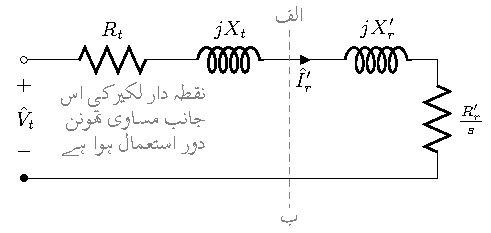
\includegraphics{figInductionMachineUsingThevenin}
\begin{tikzpicture}
\pgfmathsetmacro{\shiftX}{5cm}
\draw (0,0) to [short,o-] ++(0.5,0) to [resistor,l={$R_{t}$}]++(2,0) to [inductor,l={$j X_{t}$}] ++(2,0)coordinate(dashedUP) to [short,i_={$\hat{I}_r'$}] ++(0.5,0) to [inductor,l={$j X_r'$}] ++(2,0)  to [resistor,l={$\frac{R_r'}{s}$}] ++(0,-2) to [short,-*] (0,-2);
\draw[dashed] (dashedUP)++(0,0.5)node[above]{ا} --++(0,-3)node[below]{ب};
%text
\draw node at (0,-1){$\begin{aligned} &+\\ & \hat{V}_{t}\\ &- \end{aligned}$};
\draw node[right,align=right]  at (0.5,-1){\RL{نقطہ دار لکیر کی اس} \\ \RL{جانب مساوی تھونن} \\  \RL{دور استعمال ہوا ہے۔}};
\end{tikzpicture}%
\caption{تھونن دور استعمال کرنے کے بعد امالی موٹر کا مساوی دور۔}
\label{شکل_امالی_تھونن_استعمال_کرتے_ہوئے}
\end{figure}
کسی بھی مخلوط عدد\حاشیہب{complex number} کی طرح  \عددیء{Z_t} کو ایک حقیقی عدد \عددیء{R_t} اور ایک فرضی عدد \عددیء{j X_t} کا مجموعہ لکھا جا سکتا ہے۔ یہی اس مساوات میں کیا گیا ہے۔

ہم یوں امالی موٹر کے مساوی برقی دور کو شکل \حوالہ{شکل_امالی_تھونن_استعمال_کرتے_ہوئے}  کی طرح بنا سکتے ہیں جہاں سے دوری سمتیہ کی استعمال سے مندرجہ ذیل برقی رو \عددیء{\hat{I}_r'} حاصل ہوتا ہے۔
\begin{gather}
\begin{aligned}\label{مساوات_امالی_گھمتا_رو}
\hat{I}_r'&=\frac{\hat{V}_t}{R_t +  j X_t +\frac{R_r'}{s}+ j X_r'}\\
\abs{\hat{I}_r'}&=I_r'=\frac{V_t}{\sqrt{\left(R_t+\frac{R_r'}{s} \right)^2+\left(X_t+X_r' \right)^2}}
\end{aligned}
\end{gather}
چونکہ \عددیء{I_r'} کی   قیمت پر \عددیء{\hat{V}_t} کے زاویے کا کوئی اثر نہیں لہٰذا مساوی تھونن دور میں \عددیء{\hat{V}_t} کی جگہ  \عددیء{V \phase{0}} استعمال کیا جا سکتا ہے۔اس کتاب میں ایسا ہی کیا جائے گا۔ 

مساوات \حوالہ{مساوات_امالی_مروڑ_الف}  اور مساوات \حوالہ{مساوات_امالی_گھمتا_رو} سے  تین دوری مشین کی قوت مروڑ حاصل کرتے ہیں۔
\begin{gather}
\begin{aligned}\label{مساوات_امالی_تین_دور_مروڑ_الف}
T&=\frac{1}{\omega_{sm}} \frac{3 V_t^2 \left(\frac{R_r'}{s} \right)}{\left(R_t+\frac{R_r'}{s} \right)^2+\left(X_t+X_r' \right)^2}\\
&=\frac{1}{\omega_{sm}} \frac{3 V_t^2 \left(\frac{R_r'}{s} \right)}{\frac{R_r'^2}{s^2}+2 R_t \frac{R_r'}{s}+R_t^2+\left(X_t+X_r' \right)^2}
\end{aligned}
\end{gather}

اس مساوات کو شکل \حوالہ{شکل_امالی_مروڑ_بالمقابل_رفتار}  میں دکھایا گیا ہے جہاں موٹر کی رفتار کو معاصر رفتار کی نسبت سے دکھایا گیا ہے۔موٹر ازخود گھومتے مقناطیسی موج کے رخ گھومتی ہے اور اس کی رفتار معاصر رفتار سے  کم رہتی ہے۔زیادہ سرکاو پر موٹر کی کارگزاری  خراب ہو جاتی ہے۔ اسی لئے  لگاتار استعمال میں موٹر  تقریباً پانچ فی صد سے کم سرکاو پر چلائی جاتی ہے بلکہ ان کی بناوٹ یوں کی جاتی ہے کہ امالی موٹر اپنی بناوٹی طاقت تقریباً پانچ فی صد سے کم سرکاو پر مہیا کرتی ہو۔ 

اگر موٹر کو زبردستی ساکن لچھوں کے گھومتے مقناطیسی موج کے رخ معاصر رفتار سے زیادہ رفتار پر گھمایا جائے تو یہ ایک جنریٹر کے طور پر کام کرنے شروع ہو جائے گی۔ایسا کرنے کے لئے بیرونی میکانی طاقت درکار ہو گی ۔اگرچہ امالی مشین عام طور پر بطور جنریٹر استعمال نہیں ہوتی البتہ ہوا سے برقی طاقت کی پیداوار میں انہیں بطور جنریٹر  استعمال کیا جانے لگا ہے۔
\begin{figure}
\centering
%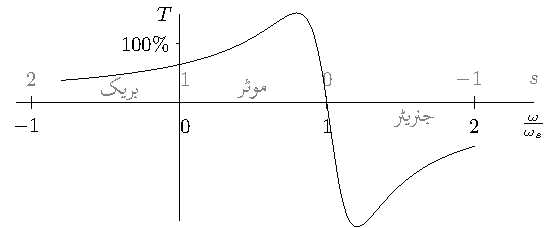
\includegraphics{figInductionTorqueSlip}
\begin{tikzpicture}[x=5cm,y=5cm]
\pgfmathsetmacro{\shiftX}{5cm}
%axis
\draw(0,0.3)node[left]{$T$}--(0,-0.4);
\draw(-0.55,0)--(1.2,0);
\draw (0,0.2)--++(-0.01,0)node[left]{$\SI{100}{\percent}$};
%
\foreach \a in {-0.5,0,0.5,1}{
\draw (\a,0.02)--++(0,-0.04); }
\foreach \a/\b in {-0.52/-1,0.02/0,0.5/1,1/2}{
\draw node at (\a,-0.08){$\b$};}
\foreach \a/\b in {-0.5/2,0.02/1,0.5/0,0.98/-1}{
\draw node[] at (\a,0.08){$\b$}; }
%
\draw node at (1.2,-0.08){$\tfrac{\omega}{\omega_s}$};
\draw node[] at (1.2,0.08){$s$};
\draw node[] at (0.8,-0.05){جنریٹر};
\draw node[] at (0.25,0.05){موٹر};
\draw node[] at (-0.2,0.05){روک};
%
\def\Rr{0.144}
\draw[scale=0.5,domain=-0.8:2,samples=50,smooth,variable=\x] plot ({\x},{(\Rr/(1-\x))/((0.113+\Rr/(1-\x))^2+(0.49+0.209)^2)});
\end{tikzpicture}
\caption{امالی موٹر کی قوت مروڑ بالمقابل سرکاو۔}
\label{شکل_امالی_مروڑ_بالمقابل_رفتار}
\end{figure}

شکل \حوالہ{شکل_امالی_مروڑ_بالمقابل_رفتار} میں منفی رفتار بھی دکھائی گئی ہے جہاں سرکاو کی قیمت اکائی سے زیادہ ہے۔ موٹر کو ساکن لچھوں کے گھومتی مقناطیسی دباو کی موج کے مخالف رخ گھمانے سے ایسا ہو گا۔ چلتی  موٹر کو جلد ساکن کرنے کے لئے ایسا کیا جاتا ہے۔تین دوری موٹر پر لاگو کسی دو برقی دباو کو آپس میں تبدیل کرنے سے موٹر کے ساکن لچھوں کے گھومتی مقناطیسی موج یکدم مخالف رخ گھومنا شروع ہو جاتی ہے جبکہ موٹر ابھی پہلے رخ گھوم رہی ہوتی ہے۔اس طرح موٹر جلد آہستہ ہوتی ہے اور جیسے ہی موٹر رک کر دوسرے رخ گھومنا چاہتی ہے اس پر لاگو برقی دباو منقطع کر دیا جاتا ہے۔امالی موٹر یوں ریل  گاڑی میں عموماً بطور \اصطلاح{روک}\فرہنگ{روک}\حاشیہب{brake} (بریک) استعمال کی جاتی ہے۔

امالی مشین \عددیء{s<0} کی صورت میں بطور جنریٹر، \عددیء{0<s<1} کی صورت میں بطور موٹر اور \عددیء{1<s} کی صورت میں بطور روک کام کرتی ہے۔

امالی موٹر کی زیادہ سے زیادہ قوت مروڑ مساوات \حوالہ{مساوات_امالی_تین_دور_مروڑ_الف}  سے  حاصل کی جا سکتی ہے۔قوت مروڑ اسی لمحہ زیادہ سے زیادہ ہو گی جب گھومتے حصے کو زیادہ سے زیادہ طاقت میسر ہو۔زیادہ سے زیادہ طاقت منتقل کرنے کے مسئلہ\فرہنگ{مسئلہ!زیادہ سے زیادہ طاقت کی منتقلی}\حاشیہب{maximum power theorem}\فرہنگ{theorem!maximum power transfer} کے مطابق مزاحمت \عددیء{\tfrac{R_r'}{s}} میں طاقت کا ضیاع اس صورت زیادہ سے زیادہ ہو گا جب (شکل \حوالہ{شکل_امالی_تھونن_استعمال_کرتے_ہوئے} میں) اس کی قیمت باقی سلسلہ وار جڑی  اجزاء کی قیمت کے برابر ہو:
\begin{align}\label{مساوات_امالی_زیادہ_طاقت_منتقلی_شرط}
\frac{R_r'}{s}=\abs{R_t+j X_t+j X_r'}=\sqrt{R_t^2+\left(X_t+X_r'\right)^2}
\end{align}
اس مساوات سے زیادہ سے زیادہ طاقت پر سرکاو \عددیء{s_z} حاصل ہو گا۔
\begin{align}\label{مساوات_امالی_زیادہ_طاقت_پر_سرک}
s_z=\frac{R_r'}{\sqrt{R_t^2+\left(X_t+X_r'\right)^2}}
\end{align}
مساوات \حوالہ{مساوات_امالی_تین_دور_مروڑ_الف}  کی نسب نما میں \عددیء{R_t^2+(X_t+X_r')^2} کی جگہ  مساوات \حوالہ{مساوات_امالی_زیادہ_طاقت_منتقلی_شرط}  کا مربع استعمال کرتے ہوئے زیادہ سے زیادہ قوت مروڑ \عددی{T_z} حاصل ہو گی:
\begin{gather}
\begin{aligned}
T_z&=\frac{1}{\omega_{sm}} \frac{3 V_t^2 \left(\frac{R_r'}{s} \right)}{\frac{R_r'^2}{s^2}+2 R_t \frac{R_r'}{s}+\frac{R_r'^2}{s^2}}\\
&=\frac{1}{\omega_{sm}} \frac{3 V_t^2 }{2 \left(R_t+\frac{R_r'}{s} \right)}\\
&=\frac{1}{\omega_{sm}} \frac{3 V_t^2}{2 \left(R_t+\sqrt{R_t^2+\left(X_t+X_r' \right)^2} \right)}
\end{aligned}
\end{gather}
درج بالا کے حصول میں آخری قدم پر مساوات \حوالہ{مساوات_امالی_زیادہ_طاقت_منتقلی_شرط} کا استعمال دوبارہ کیا گیا۔

اس مساوات کے مطابق امالی موٹر کی زیادہ سے زیادہ قوت مروڑ اس کے گھومتے لچھوں کی  مزاحمت پر منحصر نہیں ہو گی۔ یہ ایک اہم معلومات ہے جسے استعمال کر کے امالی موٹر کی زیادہ سے زیادہ قوت مروڑ درکار رفتار پر  حاصل کی جا سکتی ہے۔آئیں دیکھتے ہیں کہ ایسا کس طرح کیا جاتا ہے۔
\begin{figure}
\centering
%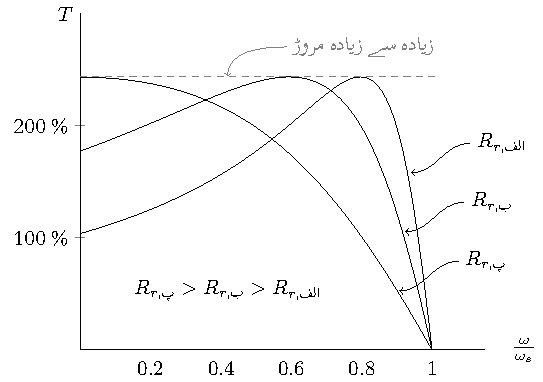
\includegraphics{figInductionTorqueSlipRotorResistanceIncreased}
\begin{tikzpicture}
\begin{axis}[
	axis lines=middle,
%	axis y line=middle,
	axis line style=-,
	xmax=1.15,
	ymax=0.75,
	ytick={0.25,0.5},
	yticklabels={$\SI{100}{\percent}$,$\SI{200}{\percent}$},
	xtick style={draw=none},
	ylabel={$T$},
	xlabel={$\tfrac{\omega}{\omega_s}$},
	every axis x label/.style={
    at={(ticklabel* cs:1.05)},
    anchor=west,
},
every axis y label/.style={
    at={(ticklabel* cs:1.00)},
    anchor=east,
},
]
\foreach \Rr in {0.144,0.288,0.72}{
\addplot[black,domain=0:1,samples=100,]{(\Rr/(1-x))/((0.113+\Rr/(1-x))^2+(0.49+0.209)^2)};}
%
\end{axis}
\draw [dashed] (0,4.63)--++(6,0);
\draw[<-] (2.5,4.63) to [out=90,in=180]++(1,0.5)node[right]{\RL{زیادہ سے زیادہ مروڑ}};
\draw[<-] (5.6,3) to [out=0,in=180]++(1,0.5)node[right]{$R_{r,\textup{ا}}$};
\draw[<-] (5.5,2) to [out=0,in=180]++(1,0.5)node[right]{$R_{r,\textup{ب}}$};
\draw[<-] (5.4,1) to [out=0,in=180]++(1,0.5)node[right]{$R_{r,\textup{ج}}$};
\draw node at (2.5,1){$R_{r,\textup{ج}} > R_{r,\textup{ب}} > R_{r,\textup{ا}}$};
\end{tikzpicture}%
\caption{بیرونی مزاحمت  کا قوت مروڑ بالمقابل سرکاو کے خطوط پر اثرات۔}
\label{شکل_امالی_بیرونی_مزاحمت_اور_مروٹ}
\end{figure}

امالی موٹر کے گھومتے لچھوں کے برقی سروں کو \اصطلاح{سرک چھلوں}\فرہنگ{سرک چھلے}\حاشیہب{slip rings}\فرہنگ{slip rings} کے ذریعہ باہر نکالا جاتا ہے\حاشیہد{شکل  کے نمونے پر۔} جہاں ان کے ساتھ سلسلہ وار بیرونی مزاحمت جوڑی جاتی ہے۔اس طرح گھومتے لچھوں کی کل مزاحمت بڑھ کر \عددیء{R_r + R_{\textup{بیرونی}}} ہو جاتی ہے۔ ایسا کرنے سے مساوات \حوالہ{مساوات_امالی_زیادہ_طاقت_منتقلی_شرط}  کے مطابق زیادہ سے زیادہ قوت مروڑ نسبتاً زیادہ سرکاو یعنی کم زاویائی رفتار پر حاصل ہو گی۔ شکل \حوالہ{شکل_امالی_بیرونی_مزاحمت_اور_مروٹ} کے مطابق مزاحمت \عددیء{R_{r,\textup{ج}}} استعمال کرتے ہوئے ساکن موٹر چالو ہوتے  وقت زیادہ سے زیادہ قوت مروڑ دے گی۔اس طرح بوجھ بردار موٹر ساکن حالت سے ہی زیادہ بوجھ اٹھانے کے قابل ہو گی۔بیرونی مزاحمت استعمال کیے بغیر یا کم بیرونی مزاحمت، مثلاً \عددیء{R_{r,\textup{ا}}}، استعمال کرتے ہوئے ساکن موٹی کی قوت مروڑ نسبتاً بہت کم ہو گی۔  چونکہ زیادہ سرکاو پر موٹر کی کارگزاری خراب ہوتی ہے لہٰذا اس طرح موٹر کو زیادہ دیر نہیں چلایا جاتا اور جیسے ہی اس کی رفتار بڑھ جاتی ہے، اس سے  بیرونی مزاحمتیں منقطع کر کے گھومتے لچھوں کے برقی سرے کسر دور کر دیے جاتے ہیں۔

\ابتدا{مثال}
صفحہ \حوالہصفحہ{مثال_امالی_ستارہ_چھ_قطب_پندرہ_کلو_واٹ} پر مثال \حوالہ{مثال_امالی_ستارہ_چھ_قطب_پندرہ_کلو_واٹ}  میں دی گئی امالی موٹر استعمال کریں اور رگڑ سے طاقت کے ضیاع کو نظر انداز کریں۔
\begin{itemize}
\item
اگر موٹر درکار وولٹ اور تعداد  پر تین فی صد سرکاو پر چل رہی ہو تب  ساکن لچھے میں گھومتے لچھے کے حصہ کا برقی رو \عددیء{I_r'} اور مشین کی اندرونی میکانی طاقت اور قوت مروڑ حاصل کریں۔
\item
موٹر کی زیادہ سے زیادہ اندرونی پیدا قوت مروڑ اور اس قوت مروڑ پر موٹر کی رفتار حاصل کریں۔
\item
موٹر چالو ہونے کے لمحہ پر قوت مروڑ اور اس لمحہ پر \عددیء{I_r'}  حاصل کریں۔ 
\end{itemize}

حل:
\begin{itemize}
\item
 یک دوری  برقی دباو \عددیء{\tfrac{415}{\sqrt{3}}=239.6}  استعمال کرتے ہوئے مساوات \حوالہ{مساوات_امالی_تھونن_متغرات}  کی مدد سے درج ذیل ہو گا۔
\begin{align*}
Z_t&=\frac{\left(0.5+j 0.99 \right) j 22}{0.5+j 0.99+j 22}=0.4576+j 0.9573\\
\hat{V}_t&=\frac{j 22 \times 239.6 \phase{0\degree}}{0.5+j 0.99+j 22}=229.2\phase{1.246\degree}
\end{align*}
مساوات \حوالہ{مساوات_امالی_گھمتا_رو}  میں  تین فی صد سرکاو پر \عددیء{\tfrac{R_r'}{s}=10.3333}  استعمال کرتے ہوئے درج ذیل ہو گا۔
\begin{align*}
\hat{I}_r'&=\frac{229.2 \phase{1.246\degree}}{0.4576+j 0.9573+10.3333+j 0.34}=21.1\phase{-5.6\degree}\\
I_r'&=\abs{\hat{I}_r'}=\SI{21.1}{\ampere}
\end{align*}
یہاں رک کر تسلی کر لیں کہ مندرجہ بالا مساوات میں \عددیء{229.2\phase{1.246\degree}} کی جگہ \عددیء{229.2\phase{0\degree}} استعمال کرنے سے \عددیء{I_r'} کی  قیمت تبدیل نہیں ہوتی ہے۔

مساوات \حوالہ{مساوات_امالی_تین_دور_میکانی_طاقت_بالمقابل_سرک_الف}  اور \حوالہ{مساوات_امالی_تین_دور_میکانی_طاقت_اور_رفتار}  کی مدد سے طاقت اور قوت مروڑ حاصل کرتے ہیں۔
\begin{align*}
p_m&=\frac{3\times 21.1^2\times 0.31}{0.03} \times (1-0.03)=\SI{13387.46}{\watt}\\
T&=\frac{13387.46}{(1-0.03) \times 2\times \pi \times 16.66}=\SI{131.83}{\newton \meter}
\end{align*}
%
\item
مساوات \حوالہ{مساوات_امالی_زیادہ_طاقت_پر_سرک} زیادہ سے زیادہ طاقت پر سرکاو درج ذیل دیتی ہے۔
\begin{align*}
s_z=\frac{0.31}{\sqrt{0.4576^2+(0.9573+0.34)^2}}=0.1638
\end{align*}
یوں موٹر کی رفتار \عددیء{1000\times(1-0.1638)=836.2} چکر فی منٹ  ہو گی۔
\item
چالو کرتے لمحہ پر سرکاو اکائی ہو گا لہٰذا \عددیء{\tfrac{R_r'}{s}=0.31} اور یوں درج ذیل ہو گا۔
\begin{align*}
\hat{I}_r'&=\frac{229.2 \phase{1.246\degree}}{0.4576+j 0.9573+0.31+j 0.34}=152.07\phase{-58.14\degree}\\
I_r'&=\SI{152}{\ampere}
\end{align*}
اس لمحہ قوت مروڑ درج ذیل ہو گی۔
\begin{align*}
T=\frac{3 \times 152.07^2 \times 0.31}{2 \times \pi \times 16.66}=\SI{205}{\newton \meter}
\end{align*}
\end{itemize}
\انتہا{مثال}
%
\ابتدا{مثال}
دو قطب، ستارہ،  پچاس ہرٹز پر چلنے والی تین دوری امالی موٹر  \عددیء{2975} چکر فی منٹ کی رفتار پر بارہ کلوواٹ کی میکانی بوجھ سے لدی ہے۔موٹر کا سرکاو اور دھرے پر قوت مروڑ  حاصل کریں۔

حل:\quad
معاصر رفتار \عددیء{\tfrac{2}{P} f_e=\tfrac{2}{2} \times 50=50} چکر فی سیکنڈ یا \عددیء{50 \times 60=3000} چکر فی منٹ ہے۔یوں سرکاو \عددیء{s=\tfrac{3000-2975}{3000}=0.00833}  یا \عددیء{0.833} فی صد ہو گا۔ موٹر کی رفتار  \عددیء{\tfrac{2975}{60}=49.5833} چکر فی سیکنڈ ہے لہٰذا اس کے  دھرے پر قوت مروڑ  \عددیء{\tfrac{12000}{2 \times \pi \times 49.58}=\SI{38}{\newton \meter}} ہو گی۔
\انتہا{مثال}
%
\حصہ{پنجرہ نما امالی موٹر}
گھومتے لچھوں کی ساخت پر ذرا غور کرتے ہیں۔ گھومتے لچھوں کے \عددیء{N_r}  چکر ہوتے ہیں جہاں \عددیء{N_r} کوئی بھی عدد ہو سکتا ہے۔سادہ ترین صورت میں \عددیء{N_r}  ایک کے برابر ہو سکتا ہے یعنی ایک ہی چکر کا گھومتا لچھا۔اب بجائے اس کے کہ قالب میں لچھوں کے لئے شگاف بنائے جائیں اور ہر شگاف میں تانبے کی تار کا ایک چکر لپٹا جائے ہم یوں بھی کر سکتے ہیں کہ ہر شگاف میں سیدھا تانبے کا ایک سلاخ رکھ دیں اور اس طرح کے سب سلاخوں کی ایک جانب کے سروں کو تانبے کی ایک دائرہ نما سلاخ سے کسر دور کر دیں اور اسی طرح دوسری جانب کے تمام سروں کو بھی ایک تانبے کی دائرہ نما سلاخ سے کسر  دور کر دیں۔ یوں تانبے کی سلاخوں کا پنجرہ حاصل ہو گا۔اسی لئے ایسی امالی موٹر کو \اصطلاح{پنجرہ نما امالی موٹر}\فرہنگ{موٹر!پنجرہ نما}\حاشیہب{squirrel cage}\فرہنگ{squirrel cage} کہتے ہیں۔

حقیقت میں شگافوں میں پگھلا تانبا یا سلور\حاشیہب{copper, aluminium}  ڈالا جاتا ہے جو ٹھنڈا ہو کر ٹھوس ہو جاتا ہے اور قالب کو جھکڑ لیتا ہے۔دونوں اطراف کے دائرہ نما کسر دور کرنے والے چھلے بھی اسی طرح اور اسی وقت ڈھالے جاتے ہیں۔  یوں ایک مضبوط گھومتا حصہ حاصل ہوتا ہے۔ اسی مضبوطی کی وجہ سے  پنجرہ نما امالی موٹر بہت مقبول ہوئی ہے۔ ایسی موٹریں سالوں تک بغیر دیکھ بھال  کام کرتی ہیں اور روز مرہ  زندگی میں ہر جگہ پائی جاتی ہیں۔گھروں میں پانی کے پمپ اور پنکھے انہیں سے چلتے ہیں۔

\حصہ{بے بوجھ موٹر  اور جامد موٹر کے معائنہ }
امالی موٹر کی کارکردگی دو معائنوں سے معلوم کی جاتی ہے جن سے موٹر کے مساوی  دور کے اجزاء  بھی حاصل کئے جاتے ہیں۔ہم تین دوری امالی موٹر کی مثال سے ان معائنوں پر بحث کرتے ہیں۔

\جزوحصہ{بے بوجھ موٹر کا معائنہ}
یہ معائنہ بالکل ٹرانسفارمر کے بے بوجھ معائنہ کی طرح ہے۔اس میں موٹر کے ہیجان انگیز برقی رو اور بے بوجھ موٹر میں طاقت کے ضیاع کی معلومات حاصل ہوتی ہیں۔ 

اس میں  بے بوجھ امالی موٹر پر یکساں تین دوری  برقی دباو\حاشیہد{\عددیء{V_{bb}} لکھتے ہوئے لفظ بے بوجھ کے پہلے حروف ب اور ب کو زیر نوشت میں bb سے ظاہر کیا گیا ہے۔} \عددیء{V_{bb}} لاگو کر کے بے بوجھ موٹر کی برقی طاقت کا ضیاع \عددیء{p_{bb}} اور اس کے ساکن لچھے  کا ہیجان انگیز برقی رو \عددیء{I_{s,bb}} ناپا جاتا ہے۔یہ معائنہ امالی موٹر کے بناوٹی برقی دباو اور برقی تعدد پر سرانجام دیا جاتا ہے۔

بے بوجھ امالی موٹر صرف اتنی قوت مروڑ پیدا کرتی ہے جتنی رگڑ اور دیگر ضیاع طاقت کی وجہ سے درکار ہو۔اتنی کم قوت مروڑ بہت کم سرکاو پر حاصل ہو گی۔مساوات \حوالہ{مساوات_امالی_گھمتا_رو}  سے ظاہر ہے کہ بہت کم سرکاو پر  \عددیء{I_r'} بھی نہایت کم ہو گا  اور اس سے گھومتے لچھوں میں برقی طاقت کا ضیاع قابل نظر انداز ہو گا۔ اسی بات کو صفحہ \حوالہصفحہ{شکل_امالی_مشین_کا_مکمل_مساوی_دور} پر شکل \حوالہ{شکل_امالی_مشین_کا_مکمل_مساوی_دور}  کی مدد سے بھی سمجھا جا سکتا ہے جہاں  واضح ہے کہ بہت کم سرکاو پر مزاحمت \عددیء{\tfrac{R_r'}{s}} کی قیمت بہت زیادہ ہو گی اور اس کو کھلا دور سمجھا جا سکتا ہے۔ایسا کرنے سے شکل \حوالہ{شکل_امالی_بے_بار_معائنہ}-ا ملتی ہے۔

شکل \حوالہ{شکل_امالی_بے_بار_معائنہ}-ا کے متوازی اجزاء \عددیء{R_c}  اور \عددیء{j X_m} کی جگہ  مساوی سلسلہ وار جڑے اجزاء پر کرنے سے  شکل \حوالہ{شکل_امالی_بے_بار_معائنہ}-ب حاصل ہو گی۔کسی بھی امالی موٹر کی \عددیء{R_c} کی قیمت اس کی \عددیء{X_m} کی قیمت سے بہت زیادہ ہوتی ہے۔متوازی دور کی رکاوٹ \عددیء{Z_m} سے مساوی سلسلہ وار رکاوٹ \عددیء{Z_s}  حاصل کرتے ہیں:
\begin{gather}
\begin{aligned}
Z_m&=\frac{R_c j X_m}{R_c+j X_m}\\
&=\frac{R_c j X_m}{R_c+j X_m} \frac{R_c-j X_m}{R_c-j X_m}\\
&=\frac{j R_c^2 X_m +R_c X_m^2}{R_c^2+X_m^2}\\
&\approx \frac{j R_c^2 X_m +R_c X_m^2}{R_c^2} \quad \quad {\textup{چونکہ} R_c \gg X_m}\\
&=j X_m+\frac{X_m^2}{R_c}=j X_m +R_c^*=Z_s
\end{aligned}
\end{gather}
بے بوجھ ٹرانسفارمروں میں ابتدائی لچھوں کی برقی طاقت کے ضیاع کو بھی نظر انداز کیا جاتا ہے۔بے بوجھ امالی موٹروں کا ہیجان انگیز برقی رو کافی زیادہ ہوتا ہے لہٰذا ان کے ساکن لچھوں کی برقی طاقت کے ضیاع کو نظر انداز نہیں کیا جا سکتا۔بے بوجھ امالی موٹر کی \عددیء{p_{bb}} سے  تین ساکن لچھوں کا برقی ضیاع منفی کر کے میکانی ضیاع طاقت حاصل ہو گا:
\begin{align}
p_{\textup{ضیاع}}=p_{bb}-3 I_{s,bb}^2 R_s
\end{align}
میکانی طاقت کا ضیاع بے بوجھ اور بوجھ بردار موٹر کے لئے ایک جیسا  تصور کیا جاتا ہے۔
\begin{figure}
\centering
%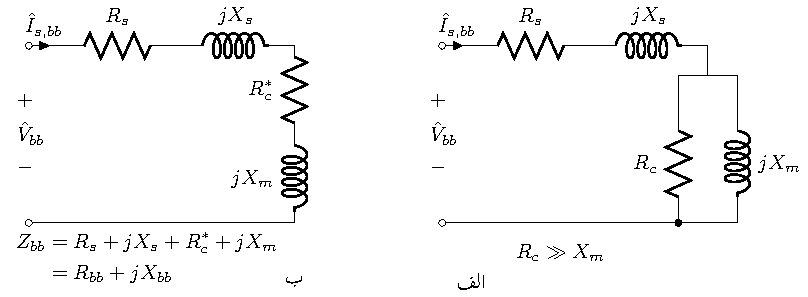
\includegraphics{figInductionUnloaded}
\begin{subfigure}{0.45\textwidth}
\centering
\begin{tikzpicture}
\draw (0,0) to [short,o-,i={$\hat{I}_{s,bb} $}] ++(0.5,0) to [resistor,l={$R_s$}]++(2,0) to [inductor,l={$j X_{s}$}] ++(2,0)coordinate(rotorStartUp) to [short,-*] ++(0,-0.5)coordinate(upperJunction) to [short] ++(-0.5,0) to [] ++(0,-0.5) to  [resistor,l_={$R_c$}] ++(0,-2) to [short,-o] ++(-4,0)coordinate(lowerLeftTerminal);
\draw (upperJunction) to [short] ++(0.5,0) to [short] ++(0,-0.5) to  [inductor,l={$j X_m$}] ++(0,-2)coordinate(rotorStartLow) to [short,-*] ++(-1,0);
%
\draw node at (0,-1.5){$\begin{aligned} &+\\ & \hat{V}_{bb}\\ &- \end{aligned}$};
\draw node at (2,-3.5){$R_c \gg X_m$};
\end{tikzpicture}
\caption{}
\end{subfigure}\hfill
\begin{subfigure}{0.45\textwidth}
\centering
\begin{tikzpicture}
\draw (0,0) to [short,o-,i={$\hat{I}_{s,bb} $}] ++(0.5,0) to [resistor,l={$R_s$}]++(2,0) to [inductor,l={$j X_{s}$}] ++(2,0) to  [resistor,l_={$R_c^{*}$}] ++(0,-1.5) to [inductor,l_={$jX_m$}] ++(0,-1.5) to [short,-o] (0,-3)coordinate(lowerLeftTerminal);
%
\draw node at (0,-1.5){$\begin{aligned} &+\\ & \hat{V}_{bb}\\ &- \end{aligned}$};
\draw node[below right] at (-0.4,-3){$\begin{aligned} Z_{bb}&=R_{s}+j X_s+R_c^*+j X_m \\ &=R_{bb} +j X_{bb}  \end{aligned}$};
\end{tikzpicture}
\caption{}
\end{subfigure}
\caption{بے بوجھ امالی موٹر کا معائنہ۔}
\label{شکل_امالی_بے_بار_معائنہ}
\end{figure}

شکل \حوالہ{شکل_امالی_بے_بار_معائنہ}-ب سے ہم درج ذیل لکھ سکتے ہیں۔
\begin{gather}
\begin{aligned}
R_{bb}&=\frac{p_{bb}}{3 I_{s,bb}^2}\\
Z_{bb}&=\frac{V_{bb}}{I_{s,bb}}\\
X_{bb}&=\sqrt{\abs{Z_{bb}}^2-R_{bb}^2}\\
X_{bb}&=X_s+X_m
\end{aligned}
\end{gather}
یوں اس معائنہ سے موٹر کی بے بوجھ متعاملیت \عددیء{X_{bb}} حاصل ہوتی ہے۔اگر کسی طرح ساکن لچھے کی متعاملیت \عددیء{X_s} معلوم ہو تب اس مساوات سے \عددیء{X_m} حاصل کی جا سکتی ہے۔اگلے معائنہ میں ہم \عددیء{X_s}  کا اندازہ لگا سکیں گے۔

\جزوحصہ{جامد موٹر کا معائنہ}
یہ معائنہ ٹرانسفارمر کے کسر دور معائنہ کی طرح ہے۔ اس میں مشین کے رستا امالوں کی معلومات حاصل ہوتی ہے۔البتہ امالی موٹر کا مسئلہ ذرا زیادہ پیچیدہ ہے۔امالی موٹر کے رستا امالہ گھومتے لچھوں میں برقی تعدد اور قالب کے سیراب ہونے پر منحصر ہوتے ہیں۔

 اس معائنہ میں امالی موٹر کے گھومتے حصہ کو حرکت کرنے سے زبردستی روک دیا جاتا ہے جبکہ ساکن لچھوں پر بیرونی برقی دباو \عددیء{V_{rk}} لاگو کر کے برقی طاقت \عددیء{p_{rk}} اور ساکن لچھوں کے برقی رو \عددیء{I_{s,rk}} ناپے جاتے ہیں۔ اصولی طور پر یہ معائنہ ان حالات کو مد نظر رکھ کر کیا جاتا ہے جن پر موٹر کی معلومات درکار ہوں۔

ساکن موٹر چالو کرنے کے  لمحہ پر موٹر کا سرکاو اکائی ہوتا ہے اور اس کے گھومتے لچھوں میں  روز مرہ تعدد \عددیء{ f_e}  کے برقی رو\حاشیہد{اس لمحہ کے برقی رو کو چھوٹی لکھائی میں وقت صفر سے منسلک کیا گیا ہے یعنی  \عددیء{t=0}} \عددیء{I_{t=0}} ہوں گے، لہٰذا اگر اس لمحہ کے نتائج درکار ہوں تب موٹر کے ساکن لچھوں پر روز مرہ تعدد، \عددیء{f_e}،   کا اتنا برقی دباو لاگو کیا جائے گا جتنے سے اس کے گھومتے لچھوں میں برقی رو \عددیء{I_{t=0}} پیدا ہو۔ اسی طرح اگر برقرار چالو حالت میں بوجھ بردار موٹر کے نتائج درکار ہوں جب موٹر کا سرکاو \عددیء{s} اور اس کے گھومتے لچھوں میں برقی رو\حاشیہد{زیر نوشت  میں \عددیء{t \to \infty} اس بات کو ظاہر کرتی ہے کہ موٹر کافی دیر سے چالو ہے اور یہ ایک برقرار رفتار تک پہنچ گئی ہے۔} \عددیء{I_{t\to \infty}} ہوتے ہیں تب معائنہ میں \عددیء{s f_e} تعدد کے برقی دباو استعمال کیے جائیں گے اور اس کی قیمت  اتنی رکھی جائے گی جتنی سے گھومتے لچھوں میں \عددیء{I_{t\to \infty}} برقی رو وجود میں آئے۔تقریباً  \عددیء{\SI{20}{\kilo \volt \ampere}} سے چھوٹی موٹروں میں برقی تعدد کے اثرات قابل نظر انداز ہوتے ہیں لہٰذا ان کا معائنہ \عددیء{f_e} تعدد کے برقی دباو پر ہی کیا جاتا ہے۔

یہاں صفحہ \حوالہصفحہ{شکل_امالی_مشین_کا_مکمل_مساوی_دور} کے شکل \حوالہ{شکل_امالی_مشین_کا_مکمل_مساوی_دور}  کو رکے (ساکن)  موٹر کے معائنہ کے نقطہ نظر سے دوبارہ دیکھتے ہیں۔رکے (ساکن) موٹر کا سرکاو اکائی ہوتا ہے۔مزید، اس معائنہ میں لاگو برقی دباو برقرار چالو موٹر پر لاگو برقی دباو سے خاصا کم ہوتا ہے۔اتنے کم لاگو برقی دباو پر قالبی ضیاع کو نظرانداز کیا جا سکتا ہے۔شکل میں  \عددیء{R_c} کو کھلے دور کرنا قالبی ضیاع کو نظرانداز کرنے کے مترادف ہے۔ایسا کرنے سے شکل \حوالہ{شکل_امالی_رکے_موٹر_معائنہ}-ا ملتا ہے۔چونکہ \عددیء{s=1} ہے لہٰذا اس شکل میں \عددیء{\tfrac{R_r'}{s}}  کو \عددیء{R_r'} لیا گیا ہے۔
\begin{figure}
\centering
%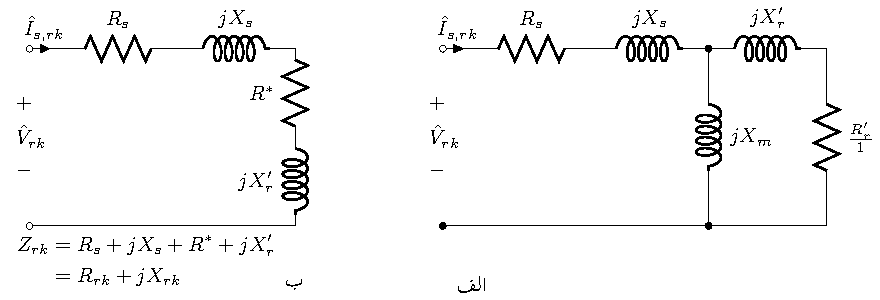
\includegraphics[width=\linewidth]{figInductionBlockedRotorTest}
\begin{subfigure}{0.50\textwidth}
\centering
\begin{tikzpicture}[scale=0.85]
\pgfmathsetmacro{\shiftX}{5cm}
\draw (0,0) to [short,o-,i={$\hat{I}_{s,rk} $}] ++(0.5,0) to [resistor,l={$R_s$}]++(2,0) to [inductor,l={$j X_{s}$}] ++(2,0)coordinate(rotorStartUpper) to  [inductor,l_={$j X_m$}] ++(0,-3)coordinate(rotorStartLow) to [short,-*] (0,-3);
\draw (rotorStartUpper) to [inductor,l={$j X_r'$},*-]++(2,0) to [resistor,l_={$\tfrac{R_r'}{1}$}] ++(0,-3) to [short,-*] (rotorStartLow);
%
\draw node at (0,-1.5){$\begin{aligned} &+\\ & \hat{V}_{rk}\\ &- \end{aligned}$};
\end{tikzpicture}
\caption{}
\end{subfigure}\hfill
\begin{subfigure}{0.40\textwidth}
\centering
\begin{tikzpicture}
\draw (0,0) to [short,o-,i={$\hat{I}_{s,rk} $}] ++(0.5,0) to [resistor,l={$R_s$}]++(2,0) to [inductor,l={$j X_{s}$}] ++(2,0) to  [resistor,l_={$R^*$}] ++(0,-1.5) to [inductor,l_={$jX_r'$}] ++(0,-1.5) to [short,-o] (0,-3)coordinate(lowerLeftTerminal);
%
\draw node at (0,-1.5){$\begin{aligned} &+\\ & \hat{V}_{rk}\\ &- \end{aligned}$};
\draw node[below right] at (-0.4,-3){$\begin{aligned} Z_{rk}&=R_{s}+j X_s+R^*+j X_r' \\ &=R_{rk} +j X_{rk}  \end{aligned}$};
\end{tikzpicture}
\caption{}
\end{subfigure}
\caption{رکے امالی موٹر کا معائنہ۔}
\label{شکل_امالی_رکے_موٹر_معائنہ}
\end{figure}

شکل  \حوالہ{شکل_امالی_رکے_موٹر_معائنہ}-ا میں \عددیء{j X_m}  اور \عددیء{(R_r'+j X_r')} متوازی جڑے ہیں جن  کی جگہ ان کی مساوی سلسلہ وار رکاوٹ پر کرنے سے شکل \حوالہ{شکل_امالی_رکے_موٹر_معائنہ}-ب حاصل ہو گی۔متوازی رکاوٹ \عددیء{Z_m} کی مساوی سلسلہ وار رکاوٹ \عددیء{Z_s}  حاصل کرتے ہیں:
\begin{gather}
\begin{aligned}
Z_m&=\frac{j X_m (R_r'+j X_r')}{R_r'+j(X_m+X_r')}\\
&=\left( \frac{j X_m R_r' -X_m X_r'}{R_r'+j(X_m+X_r')} \right) \left( \frac{R_r'-j(X_m+X_r')}{R_r'-j(X_m+X_r')}\right)\\
&=\frac{jX_m R_r'^2+X_m R_r'(X_m+X_r')-X_m X_r' R_r' +j X_m X_r'(X_m+X_r')}{R_r'^2+(X_m+X_r')^2}\\
&=\frac{X_m^2 R_r'}{R_r'^2+(X_m+X_r')^2}+\frac{j(X_m R_r'^2+X_m^2 X_r'+X_m X_r'^2)}{R_r'^2+(X_m+X_r')^2}\\
&=R_s^*+j X_s^* =Z_s
\end{aligned}
\end{gather}
ان مساوات میں \عددیء{X_m \gg R_r'} اور \عددیء{X_m \gg X_r'}  لینے سے درج ذیل حاصل ہو گا۔
\begin{align}\label{مساوات_امالی_تقریبا_مزاحمت}
R_s^*& \approx R_r' \left(\frac{X_m}{X_m+X_r'} \right)^2 \\
X_s^*&= \approx  \frac{X_m R_r'^2}{X_m^2}+\frac{X_m^2 X_r'}{X_m^2}+\frac{X_m X_r'^2}{X_m^2} \approx X_r'
\end{align}
اس معائنہ میں پیمائش کی گئی قیمتوں اور شکل \حوالہ{شکل_امالی_رکے_موٹر_معائنہ}-ب سے درج ذیل حاصل ہو گا۔
\begin{gather}
\begin{aligned}
Z_{rk} &=\frac{V_{rk}}{I_{s,rk}}\\
R_{rk}&=\frac{p_{rk}}{3 I_{s,rk}^2}\\
X_{rk}&=\sqrt{\abs{Z_{rk}}^2-R_{rk}^2}
\end{aligned}
\end{gather}
اس مساوات کے پہلے جزو میں پیمائشی برقی دباو اور برقی رو سے رکاوٹ حاصل کی گئی ہے۔ اس طرح دوسرے جزو میں مزاحمت اور تیسرے میں متعاملیت کا حساب لگایا گیا ہے۔

شکل \حوالہ{شکل_امالی_رکے_موٹر_معائنہ}-ب سے درج ذیل واضح ہے۔ 
\begin{align}
X_{rk}=X_s+X_r'
\end{align}
امالی مشین مختلف خواص کے بنائے جاتے ہیں۔عام  آدمی کی آسانی کے لئے ایسی مشینوں کی درجہ بندی کی جاتی ہے۔جدول \حوالہ{جدول_امالی_امالہ_کا_تقسیم} میں پنجرہ نما امالی موٹر کی  مختلف اقسام \عددیء{A,B,C,D} اور ایسی مشین جن کا گھومتا حصہ لچھے پر مشتمل ہو،  کی رستا متعاملیت  \عددیء{X_{rk}} کو ساکن اور گھومتے لچھوں میں  تقسیم کرنا دکھایا گیا ہے۔اس جدول کے مطابق، گھومتے لچھے والی مشین میں ساکن اور گھومتی متعاملیت ایک دوسرے کے برابر ہوتی ہیں۔
\begin{table}
\centering
\begin{tabular}{r r c c}
گھومتا حصہ &خاصیت& \عددیء{X_s} & \عددیء{X_r'}\\
\hline\\
لپٹا ہوا & کارکردگی گھومتے حصے کی مزاحمت پر منحصر&\عددیء{0.5 X_{rk}} & \عددیء{0.5 X_{rk}} \\
بناوٹ \عددیء{A} &عمومی ابتدائی قوت مروڑ، عمومی ابتدائی رو& \عددیء{0.5 X_{rk}} & \عددیء{0.5 X_{rk}} \\
بناوٹ \عددیء{B} & عمومی ابتدائی قوت مروڑ، کم ابتدائی رو&\عددیء{0.4 X_{rk}} & \عددیء{0.6 X_{rk}} \\
بناوٹ \عددیء{C} &زیادہ ابتدائی قوت مروڑ، کم ابتدائی رو &\عددیء{0.3 X_{rk}} & \عددیء{0.7 X_{rk}} \\
بناوٹ \عددیء{D} &زیادہ ابتدائی قوت مروڑ، زیادہ سرکاو &\عددیء{0.5 X_{rk}} & \عددیء{0.5 X_{rk}} 
\end{tabular}
\caption{متعاملیت کی ساکن اور گھومتے حصوں میں تقسیم۔}
\label{جدول_امالی_امالہ_کا_تقسیم}
\end{table}
شکل  \حوالہ{شکل_امالی_رکے_موٹر_معائنہ}-ب میں \عددیء{R_{rk}=R^*+R_s} ہے لہٰذا  ساکن لچھے کی مزاحمت \عددیء{R_s}  \اصطلاح{مزاحمت پیما}\فرہنگ{مزاحمت پیما}\حاشیہب{Ohm meter} کی مدد سے ناپ کر درج ذیل حاصل کیا جا سکتا ہے۔
\begin{align}
R^*=R_{rk}-R_s
\end{align}
اب \عددیء{R_r'} کو مساوات \حوالہ{مساوات_امالی_تقریبا_مزاحمت}  سے حاصل کیا جا سکتا ہے جہاں \عددیء{X_m} بے بوجھ امالی موٹر کے معائنہ میں حاصل کی جاتی ہے۔

مزاحمت پیما کی مدد سے ساکن لچھے کی مزاحمت ناپتے وقت یہ جاننا ضروری ہے کہ موٹر ستارہ یا تکونی جڑی ہے۔شکل \حوالہ{شکل_امالی_ساکن_مزاحمت_کا_حصول}  میں لچھے کو دونوں طرح جڑا دکھایا گیا ہے۔ اگر یک دوری مزاحمت \عددیء{R_s}  ہو تب ستارہ جڑی موٹر کے لئے مزاحمت پیما  \عددیء{2 R_s} مزاحمت دے گا جبکہ تکونی جڑی موٹر کے لئے یہ \عددیء{\tfrac{2}{3} R_s} مزاحمت دے گا۔
\begin{figure}
\centering
%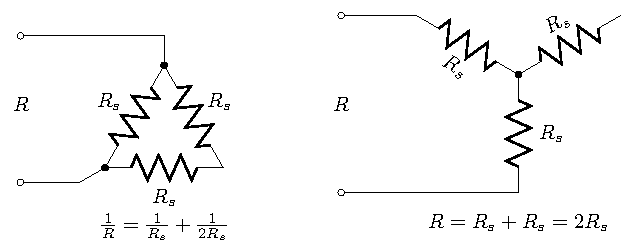
\includegraphics{figInductionStarDeltaStator}
\pgfmathsetmacro{\h}{sqrt(3)/2*2}
\pgfmathsetmacro{\hc}{\h/3}
\pgfmathsetmacro{\x}{(2/3*\h+0.5)*cos (30)}
\pgfmathsetmacro{\xsize}{2*cos(30)}
\pgfmathsetmacro{\ysize}{2*sin(30)}
\begin{subfigure}{0.50\textwidth}
\centering
\begin{tikzpicture}
\draw (0,0) to [resistor,*-,l={$R_s$}] ++(-90:2) to [short,-o] ++(180:3);
\draw (0,0) to [resistor,l={$R_s$}] ++(30:2);
\draw (0,0) to [resistor,l={$R_s$}] ++(150:2) to [short,-o]++(180:3-\xsize);
%
\draw node at (-3,+\ysize/2-1){$R$};
\draw  node at (0,-2.5){$R=R_s+R_s=2R_s$};
\end{tikzpicture}
\end{subfigure}\hfill
\begin{subfigure}{0.40\textwidth}
\centering
\begin{tikzpicture}
\draw (0,0)++(-150:2/3*\h) to [resistor,*-]++(0:2) coordinate(a) to [resistor]++(120:2)coordinate(b) to [resistor]++(-120:2);
\draw node at (-90:\hc+0.5){$R_s$};
\draw node at (30:\hc+0.5){$R_s$};
\draw node at (150:\hc+0.5){$R_s$};
\draw (-150:2/3*\h) to [short]++(-150:0.5) to [short,-o]++(180:1);
\draw (b) to [short,*-] ++(90:0.5) to [short,-o] ++(180:2.433);
\draw node at (-2.433,0.5){$R$};
\draw node at (-90:\hc+1){$\tfrac{1}{R}=\tfrac{1}{R_s}+\tfrac{1}{2R_s}$};
\end{tikzpicture}
\end{subfigure}
\caption{ستارہ اور تکونی جڑی موٹروں کی ساکن لچھوں کی مزاحمت کا مزاحمت پیما کی مدد سے حصول۔}
\label{شکل_امالی_ساکن_مزاحمت_کا_حصول}
\end{figure}

\ابتدا{مثال}
ستارہ، چار قطب، پچاس ہرٹز اور \عددیء{415} وولٹ پر چلنے والی موٹر کے معائنے کئے جاتے ہیں۔ موٹر کی بناوٹ درجہ بندی \عددیء{A}  کے مطابق ہے۔مزاحمت پیما کسی بھی دو برقی سروں کے بیچ \عددیء{0.55} اوہم جواب دیتا ہے۔بے بوجھ معائنہ \عددیء{\SI{50}{\hertz}} اور \عددیء{\SI{415}{\volt}} پر کرتے ہوئے برقی رو \عددیء{\SI{4.1}{\ampere}} اور طاقت کا ضیاع \عددیء{\SI{906}{\watt}} ناپا جاتا ہے۔جامد موٹر معائنہ  \عددیء{\SI{15}{\hertz}} اور \عددیء{\SI{50}{\volt}} پر کرتے ہوئے برقی رو \عددیء{\SI{13.91}{\ampere}} اور طاقت کا ضیاع \عددیء{\SI{850}{\watt}} ناپا جاتا ہے۔اس موٹر کا مساوی برقی دور بنائیں اور پانچ فی صد سرکاو پر اس کی اندرونی میکانی طاقت حاصل کریں۔

حل:\quad
مزاحمت پیما کے جواب سے  ستارہ موٹر کے ساکن لچھے کی مزاحمت \عددیء{R_s=\tfrac{0.55}{2}=\SI{0.275}{\ohm}} حاصل ہوتی ہے۔بے بوجھ معائنہ میں یک دوری برقی دباو \عددیء{\tfrac{415}{\sqrt{3}}=\SI{239.6}{\volt}} ہے جس سے درج ذیل حاصل ہوتے ہیں۔
\begin{align*}
R_{bb} &=\frac{906}{3 \times 4.1^2}=\SI{17.965}{\ohm}\\
\abs{Z_B}&=\frac{239.6}{4.1}=\SI{58.439}{\ohm}\\
X_{bb}&=\sqrt{58.439^2-17.965^2}=\SI{55.609}{\ohm}=X_s+X_m
\end{align*}
رکے موٹر معائنہ کے نتائج سے \عددیء{X_s} حاصل کرنے کے بعد \عددیء{X_m} حاصل ہو گی۔

ساکن لچھے کی مزاحمت میں اس برقی رو پر کل
\begin{align*}
3 I_{bb}^2 R_s=3 \times 4.1^2 \times  0.275=\SI{13.87}{\watt}
\end{align*}
برقی طاقت کا ضیاع ہو گا لہٰذا رگڑ اور دیگر ضیاع طاقت \عددیء{906-13.86=892} واٹ ہو گا۔

رکے موٹر معائنہ میں یک دوری برقی دباو \عددیء{\tfrac{50}{\sqrt{3}}=28.9} وولٹ ہیں۔ یوں درج ذیل حاصل ہوں گے۔
\begin{align*}
R_{rk}&=\frac{850}{3 \times 13.91^2}=\SI{1.464}{\ohm}\\
\abs{Z_{rk}}&=\frac{28.9}{13.91}=\SI{2.07}{\ohm}\\
X_{rk, 15}&=\sqrt{2.07^2-1.464^2}=\SI{1.46}{\ohm}
\end{align*}
اس معائنہ میں برقی تعدد \عددیء{15} ہرٹز تھا لہٰذا \عددیء{50} ہرٹز پر متعاملیت درج ذیل ہو گی۔
\begin{align*}
X_{rk,50}=\frac{50}{15} \times X_{rk,15} \approx \SI{4.9}{\ohm}
\end{align*}
درجہ بندی \عددیء{A} کی امالی موٹر میں یہ متعاملت ساکن اور گھومتے لچھے میں ایک جیسی تقسیم ہو گی:
\begin{align*}
X_s=X_r'=\frac{4.9}{2}=\SI{2.45}{\ohm}
\end{align*}
یوں درج ذیل ہو گا۔
\begin{align*}
X_m=X_{bb}-X_s=55.609-2.45=\SI{53}{\ohm}
\end{align*}
چونکہ  \عددیء{R_s=0.275} اوہم ہے  لہٰذا
\begin{align*}
R_r'=R_{rk}-R_s=1.464-0.275=\SI{1.189}{\ohm}
\end{align*}
ہو گا۔مساوی برقی دور شکل \حوالہ{شکل_امالی_موٹر_مثال_کا_دور} میں دکھایا گیا ہے۔
\begin{figure}
\centering
%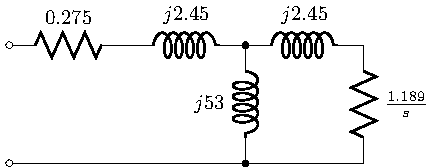
\includegraphics{figInductionMachineEquivalentCircuitExample}
\begin{tikzpicture}
\pgfmathsetmacro{\shiftX}{5cm}
\draw (0,0)  to [resistor,o-,l={$0.275$}]++(2,0) to [inductor,l={$j 2.45$}] ++(2,0)coordinate(rotorStartUp) to  [inductor,l_={$j 53$}] ++(0,-2)coordinate(rotorStartLow) to [short,*-o] ++(-4,0);
\draw (rotorStartUp)  to [inductor,*-,l={$j 2.45$}] ++(2,0) to [resistor,l={$\tfrac{1.189}{s}$}] ++(0,-2) to [short] (rotorStartLow);
\end{tikzpicture}
\caption{امالی موٹر کا مساوی برقی دور۔}
\label{شکل_امالی_موٹر_مثال_کا_دور}
\end{figure}

پانچ فی صد سرکاو پر اندرونی میکانی طاقت کی خاطر بائیں جانب کا تھونن مساوی دور استعمال کرتے ہوئے  درج ذیل ہو گا۔
\begin{align*}
V_t&=229 \phase{0.2833 \degree}\\
Z_t&=0.251+j2.343\\
\abs{\hat{I}_r'}&=\SI{11.8}{\ampere}\\
p_m&=\frac{3 \times 11.8^2 \times 0.974 \times (1-0.05)}{0.05}=\SI{7730}{\watt}
\end{align*}
\انتہا{مثال}

